\documentclass[pdflatex,sn-mathphys-num,iicol]{sn-jnl}

\usepackage[T1]{fontenc}
\geometry{text={160mm,240mm}}
\usepackage{amsmath,amssymb}
\usepackage{algorithm}
\usepackage{algpseudocode}
\algrenewcommand\algorithmicrequire{\textbf{Input:}}
\algrenewcommand\algorithmicensure{\textbf{Output:}}
\algrenewcommand{\algorithmiccomment}[1]{\hfill(#1)}
\usepackage{booktabs}
\usepackage{placeins}
\usepackage{array}
\usepackage{graphicx}
\usepackage{tikz}
\usepackage{pgfplots}
\pgfplotsset{compat=1.17}
\usetikzlibrary{arrows.meta,calc,positioning,patterns}
\hypersetup{hypertexnames=false}
\renewcommand{\topfraction}{0.9}
\renewcommand{\bottomfraction}{0.8}
\renewcommand{\textfraction}{0.07}
\renewcommand{\floatpagefraction}{0.8}
\renewcommand{\dbltopfraction}{0.9}
\renewcommand{\dblfloatpagefraction}{0.8}
\setcounter{topnumber}{3}
\setcounter{bottomnumber}{2}
\setcounter{totalnumber}{5}
\setcounter{dbltopnumber}{3}
\setlength{\floatsep}{9pt plus 3pt minus 2pt}
\setlength{\textfloatsep}{10pt plus 3pt minus 2pt}
\setlength{\dblfloatsep}{9pt plus 3pt minus 2pt}
\setlength{\dbltextfloatsep}{10pt plus 3pt minus 2pt}
\newcommand{\ci}[3]{\begin{tabular}[c]{@{}c@{}}$#1$\\{}[$#2$, $#3$]\end{tabular}}
\newcommand{\cib}[3]{{\boldmath\ci{#1}{#2}{#3}}}
\newcommand{\cit}[3]{\begin{tabular}[t]{@{}c@{}}$#1$\\{}[$#2$, $#3$]\end{tabular}}
\newcommand{\cibt}[3]{{\boldmath\cit{#1}{#2}{#3}}}
\newcommand{\scl}{SCL}
\newcommand{\aob}{AOB}
\newcommand{\twol}[2]{\begin{tabular}[c]{@{}l@{}}#1\\#2\end{tabular}}

\makeatletter
\def\email#1{\global\advance\emailcnt by 1\relax
\if@corauemail
  \ifx\corrauthemail\@empty\g@addto@macro\corrauthemail{\textcolor{blue}{#1}}%
  \else\g@addto@macro\corrauthemail{;\ \textcolor{blue}{#1}}\fi
\else
  \ifx\authemail\@empty\g@addto@macro\authemail{\textcolor{blue}{#1}}%
  \else\g@addto@macro\authemail{;\ \textcolor{blue}{#1}}\fi
\fi}
\makeatother

\makeatletter\setlength{\@fptop}{0pt}\setlength{\@dblfptop}{0pt}\makeatother
\makeatletter
\renewcommand\section{\@startsection{section}{1}{\z@}{-10pt \@plus -3pt \@minus -2pt}{6pt}{\sectionfont}}
\renewcommand\subsection{\@startsection{subsection}{2}{\z@}{-9pt \@plus -3pt \@minus -2pt}{4pt}{\subsectionfont}}
\makeatother
\begin{document}

\title[Self-Calibrating Control Layer for Multi-Object Trackers]{Training-Free Self-Calibrating Control Layer for Heterogeneous Multi-Object Trackers}

\author*[2]{\fnm{Ahmed Gouda} \sur{Ismail}}\email{a7medgouda1@gmail.com}
\author[1]{\fnm{Tarek Ahmed} \sur{Mahmoud}}\email{tarek.mohamed@eui.edu.eg}
\author[2]{\fnm{Mohamed S.} \sur{Mohamed}}\email{mohamedms@mtc.edu.eg}

\affil[1]{\orgdiv{Computer Engineering Department}, \orgname{Egypt University of Informatics}, \orgaddress{\city{Cairo}, \country{Egypt}}}
\affil*[2]{\orgdiv{Computer Engineering and Artificial Intelligence Department}, \orgname{Military Technical College}, \orgaddress{\city{Cairo}, \country{Egypt}}}

\abstract{Multi-object trackers rely on score thresholds tuned for one detector. When the detector is replaced, retrained, or compressed, its scores shift, and the tuned thresholds silently stop fitting. This paper proposes a training-free self-calibrating control layer (\scl{}) between an unchanged detector and tracker. \scl{} splits the logits of recent scores twice with Otsu's method and classifies the stream as clean or noisy, without labels or future frames. Its novelty is selective, host-aware adaptation. On clean streams it keeps the tracker's scores and lowers a threshold only if it would reject the confident detections; on noisy streams it selects and rescores the detections and sets the thresholds. It acts through four published tracker settings and passes on weak detections that continue tracks, so one frozen configuration serves single-stage and two-stage trackers. It was evaluated on seven trackers, four detection sources, and three datasets; changes are relative to the tracker alone. When detector scores were halved, two trackers fell to zero higher order tracking accuracy (HOTA); with \scl{} both recovered at least 97\% of it. With a replacement detector, RT-DETR-L, \scl{} raised the multiple object tracking accuracy (MOTA) of ByteTrack and BoT-SORT by 12.6\% and 16.3\% and cut their identity switches by 43\% and 47\%, respectively. It also raised the HOTA of PD-SORT, unseen during design, by 0.9\%, and kept four well-matched trackers within 0.1\%. \scl{} adds on average no more than 2.95 ms per frame on an ordinary processor, so a detector can be replaced or retrained without retuning the tracker.}



\keywords{multi-object tracking, tracking by detection, detector confidence calibration, online adaptation, Otsu thresholding, real-time image processing}

\maketitle

% --- sections/01_introduction
\section{Introduction}\label{sec:intro}

Multi-object tracking (MOT) finds every object of interest in a video and gives each one an
identity number (ID) that stays the same over time. It is used in surveillance, driving, and drone
systems \cite{zhu2022visdrone}, where results are needed with little delay. Most
MOT systems follow the tracking-by-detection design \cite{adzemovic2026survey}: in each frame, a
detector returns candidate boxes with confidence scores, and a tracker links them into tracks, one
per object \cite{bewley2016sort,zhang2022bytetrack,cao2023ocsort}. The tracker uses a box only if
its score passes a fixed threshold. A two-stage tracker, such as ByteTrack, also uses lower-score
boxes in a second step to continue unmatched tracks \cite{zhang2022bytetrack}; a single-stage
tracker, such as OC-SORT, ignores every box below one threshold \cite{cao2023ocsort}.

In real systems the detector is often replaced, retrained, or compressed, while the tracker keeps
the thresholds that their authors set for another detector. Detector scores are not calibrated across
models and conditions \cite{kuppers2020detcalib}, so a new detector usually gives scores on a
different scale, and nothing in the system notices. The effect can be large: halving the scores of
a published detector reduces the higher order tracking accuracy (HOTA) \cite{luiten2021hota} of two
well-known trackers to 0, because no detection passes their thresholds (Sect.~\ref{sec:shift}). For example, ByteTrack in
its official setting starts a track only from a box with a score of at least 0.7; a car that the
original detector scored 0.9 now gets 0.45, so ByteTrack never starts a track, and its HOTA falls
from 67.70 to 0. \scl{} finds from the scores themselves that the confident group now begins
lower and lets it reach the tracker again, and ByteTrack reaches 66.17 HOTA again, with no labels and no change to its code.
Retuning every tracker for every detector needs labels, which a working system usually does not
have. Adaptive-threshold methods are each built into one tracker
\cite{ma2023adaptivebytetrack,shim2024adaptrack,act2026adaptive}, score calibration needs
labelled data \cite{kuppers2020detcalib}, and adaptive inference methods learn their settings for
one model \cite{han2022dynamic}.

This paper presents a self-calibrating control layer (\scl{}) that sits between a detector and a
tracker that are both kept fixed (frozen): their code, weights, and stored settings are
unchanged. We call the tracker that \scl{} serves the \emph{host}. The novelty of \scl{} is
\emph{selective, host-aware adaptation}. It is selective because it first decides, from the
detector scores alone and without labels, whether the scores of the stream fit the host at all:
when most higher scores of recent frames form a clearly confident group, the stream is clean, and
the host keeps its scores and, unless they would reject the confident group, its thresholds. Only
when many scores are uncertain does \scl{} take control: it chooses which candidates reach the
host, gives them new scores, and sets the host's thresholds for the frame. It is host-aware because
every action is expressed in the host's own terms: four published settings of the host, the host
contract (Sect.~\ref{sec:contract}), tell the layer where the host's thresholds lie and whether it
has a low-score step, so the same frozen rules serve single-stage and two-stage trackers.

With halved detector scores, \scl{} restored two trackers from 0 to about 66 HOTA; with other
detectors, it raised the multiple object tracking accuracy (MOTA) of two-stage trackers by up to
24.7 points and cut their identity switches by 43\% to 56\%, while well-matched strong trackers
stayed within 0.06 HOTA points of their own accuracy.

The main contributions are:
\begin{enumerate}
\item \emph{Selective adaptation.} A label-free, causal test of detector--tracker compatibility:
      nested Otsu splits of recent logits and a whole-stream majority rule decide whether to act,
      so a well-matched system is left as it is and a mismatched one is corrected
      (Sects.~\ref{sec:calib}--\ref{sec:choice}).
\item \emph{Host-aware adaptation.} A host contract of four published values through which one
      fixed configuration sets the thresholds, scores, and matching tolerance of unchanged
      single-stage and two-stage trackers, with a track-guided recovery of weak detections for
      trackers that lack a low-score step (Sects.~\ref{sec:rescue}--\ref{sec:contract}).
\item \emph{Evidence for compatibility.} An evaluation of one frozen configuration on seven
      trackers, four detection sources, and three datasets, with paired bootstrap intervals,
      comparisons with adaptive thresholds and the published ACT method, a component ablation and a
      parameter sensitivity analysis (Sect.~\ref{sec:results}), the recorded development path
      (Sect.~\ref{sec:development}), and a cost of about 3 ms per frame on an ordinary processor
      (central processing unit, CPU) (Sect.~\ref{sec:discussion}).
\end{enumerate}

Section~\ref{sec:related} presents the datasets, evaluation metrics, and related work.
Section~\ref{sec:method} describes the proposed \scl{} framework, while
Section~\ref{sec:development} details its development and refinement. Section~\ref{sec:results}
presents the experimental results and evaluation. Finally, Sections~\ref{sec:discussion}
and~\ref{sec:conclusion} discuss the practical implications and summarize the main findings and
future research directions, respectively.
% --- sections/02_background
\section{Background and Related Work}\label{sec:related}

\subsection{Datasets}\label{sec:data}
Three public datasets are used. \emph{MOT17} \cite{milan2016mot16} contains 14 sequences of
people filmed with static and moving cameras. As is common, the second half of each of the seven
training sequences, called val-half (2,652 frames), is used for evaluation \cite{zhang2022bytetrack},
with the published YOLOX-X detections \cite{ge2021yolox} at the two published emission floors, the
lowest scores emitted, of 0.01 and 0.1. To study score changes directly, these scores were also
changed before the tracker by four transforms that keep their order: cubing ($s^3$), halving
($0.5\,s$), and logit temperatures $T=2$ and $T=0.5$, which divide the logit (log-odds, Sect.~\ref{sec:problem}) of each score by $T$.
\emph{KITTI tracking} \cite{geiger2012kitti} has 21 training sequences (8,008 frames) recorded from
a car and is scored on cars and pedestrians; here the trackers run with two other detectors,
YOLOv8n \cite{jocher2023yolov8} and RT-DETR-L \cite{zhao2024rtdetr}, and keep thresholds that were
set for other detectors. \emph{UAVDT} \cite{du2018uavdt} contains drone videos of vehicles; its 20
test sequences (16,592 frames) are used with ByteTrack, YOLOv8n, and RT-DETR-L.

MOT17 with four trackers, KITTI, and the score transforms were development data, looked at while
\scl{} was designed. Two predeclared external trackers, PD-SORT and Hybrid-SORT, were chosen in
advance and run once with the frozen configuration on the detections released by their authors on
MOT17 val-half. The held-out UAVDT test split was also run once, after a written plan. Each
external host was checked against its authors' number: EXACT within 0.2 HOTA points, CLOSE within
1.0.

\subsection{Evaluation metrics}\label{sec:metrics}
HOTA \cite{luiten2021hota}, the main metric, balances finding the objects and keeping their
identities,
\begin{equation}
\mathrm{HOTA}=\frac{1}{19}\sum_{\alpha}\sqrt{\mathrm{DetA}_\alpha\,\mathrm{AssA}_\alpha},
\label{eq:hota}
\end{equation}
where $\mathrm{DetA}_\alpha$ and $\mathrm{AssA}_\alpha$ are the detection and association accuracy
at the localization threshold $\alpha=0.05,0.10,\dots,0.95$.

MOTA \cite{bernardin2008clear} and
IDF1 \cite{ristani2016idf1} are
\begin{align}
\mathrm{MOTA}&=1-\frac{\mathrm{FN}+\mathrm{FP}+\mathrm{IDS}}{\mathrm{GT}},\label{eq:mota}\\
\mathrm{IDF1}&=\frac{2\,\mathrm{IDTP}}{2\,\mathrm{IDTP}+\mathrm{IDFP}+\mathrm{IDFN}},\label{eq:idf1}
\end{align}
where FN are missed objects (false negatives), FP false positives, IDS identity switches (an
object's ID changes), and GT the number of ground-truth boxes; IDTP, IDFP, and IDFN count boxes
after each ground-truth track is matched to at most one output track.

All metrics are computed
with TrackEval (commit 12c8791) and the official ground truth \cite{dendorfer2021motchallenge};
KITTI HOTA is averaged over cars and pedestrians, and on UAVDT all vehicles form one class and
predictions in ignored regions are removed. HOTA, MOTA, and IDF1 are in percent, and differences
in points.

All comparisons are paired: each tracker runs alone and with \scl{} on the same sequences and
detections. Paired bootstrap resampling of whole sequences \cite{efron1993bootstrap}, 10,000 times
with seed 42, gives a 95\% interval (2.5--97.5 percentiles) for each difference, which is called
significant when its interval does not include zero.

\subsection{Related work}\label{sec:survey}
\emph{Tracking by detection.}\label{sec:hosts} SORT matches Kalman-filter predictions to new
detections by their overlap \cite{bewley2016sort}; ByteTrack added a second step that uses
low-score detections to continue tracks \cite{zhang2022bytetrack}; OC-SORT uses one score
threshold \cite{cao2023ocsort}. Their thresholds were tuned for one detector, usually YOLOX
\cite{ge2021yolox}. Many recent trackers improve association with trained or domain-specific
parts \cite{li2024fdbtrack,bao2024graphmatching,zhang2025sinkhorn,ding2025remot,liang2024motiontrack,sun2026bsr},
which change or retrain the tracker; \scl{} keeps both the tracker and the detector unchanged.
Seven published trackers serve as hosts in this study, each with the authors' code and published
configuration: ByteTrack, BoT-SORT \cite{aharon2022botsort}, OC-SORT, SparseTrack
\cite{liu2025sparsetrack}, BoostTrack \cite{stanojevic2024boosttrack}, PD-SORT
\cite{wang2025pdsort}, and Hybrid-SORT \cite{yang2024hybridsort}. ByteTrack is used with the
thresholds that its authors used on MOT17 (official setting) and with the defaults of the
Ultralytics library, which also provides BoT-SORT (library setting).

\emph{Adaptive thresholds.} Adaptive ByteTrack sets ByteTrack's threshold from each frame
\cite{ma2023adaptivebytetrack}, AdapTrack adapts its matching thresholds \cite{shim2024adaptrack},
and ACT sets the high and low thresholds from the first quartile and the number of the current
scores \cite{act2026adaptive}. ConfTrack weights the Kalman update and the matching cost by the
score \cite{jung2024conftrack}, and PlugTrack blends motion predictors with a trained network
\cite{kim2026plugtrack}.

\emph{Comparison.} Table~\ref{tab:compare} compares \scl{} with the adaptive-thresholding and
score-calibration methods. The adaptive-thresholding methods act in every frame, read only the
current frame or each box, and are built into one tracker; calibration acts on every score and
needs labelled data. \scl{} differs in three ways. It is selective: it first decides, from the
scores of past frames, whether to act at all, and leaves a well-matched tracker as it is. It is
host-aware: it reads the tracker's published settings and serves several unchanged single-stage
and two-stage trackers through them. And it needs neither labels nor trained parts; its new scores
encode decisions for the tracker's thresholds rather than calibrated probabilities
(Sect.~\ref{sec:choice}). It is also tested as one frozen configuration under score changes and on
external systems, and against ACT on the same detections (Sect.~\ref{sec:baselines}).

% --- tables/tab_compare
\begin{table*}[!tp]
\caption{\scl{} compared with adaptive-thresholding and score-calibration methods. Each row is one method; the columns give what it changes, what information it uses, whether it needs labels or trained parts, when it acts, and where it runs. ReID: re-identification network.}
\label{tab:compare}
\centering\footnotesize
\setlength{\tabcolsep}{3pt}
\begin{tabular}{@{}>{\raggedright\arraybackslash}p{23mm}>{\raggedright\arraybackslash}p{28mm}>{\raggedright\arraybackslash}p{28mm}>{\raggedright\arraybackslash}p{19mm}>{\raggedright\arraybackslash}p{24mm}>{\raggedright\arraybackslash}p{25mm}@{}}
\toprule
Method & What is adapted & Information used & Labels or trained parts & When it acts & Where it works\\
\midrule
\multicolumn{6}{@{}l}{\textit{Adaptive thresholding}}\\
Adaptive ByteTrack \cite{ma2023adaptivebytetrack} & high/low score split & scores of the current frame & none & every frame & inside ByteTrack\\
AdapTrack \cite{shim2024adaptrack} & matching thresholds & current frame & ReID network & every frame & its own tracker\\
ACT \cite{act2026adaptive} & high and low thresholds, chosen from preset levels & first quartile and number of the current scores & none & every frame & inside the tracker\\
ConfTrack \cite{jung2024conftrack} & Kalman update and matching cost & score of each box & ReID network & every box & its own tracker\\
\addlinespace[3pt]
\multicolumn{6}{@{}l}{\textit{Score calibration}}\\
K{\"u}ppers et al.\ \cite{kuppers2020detcalib} & detector scores, mapped to probabilities & labelled data & calibration map & every score & detector output\\
\addlinespace[3pt]
\multicolumn{6}{@{}l}{\textit{This paper}}\\
\scl{} & candidates, scores, thresholds, matching tolerance & logits of past frames; host contract & none & only when the scores are noisy (clean: thresholds capped) & between a detector and unchanged trackers\\
\bottomrule
\end{tabular}
\end{table*}

\begin{figure*}[t]
\centering
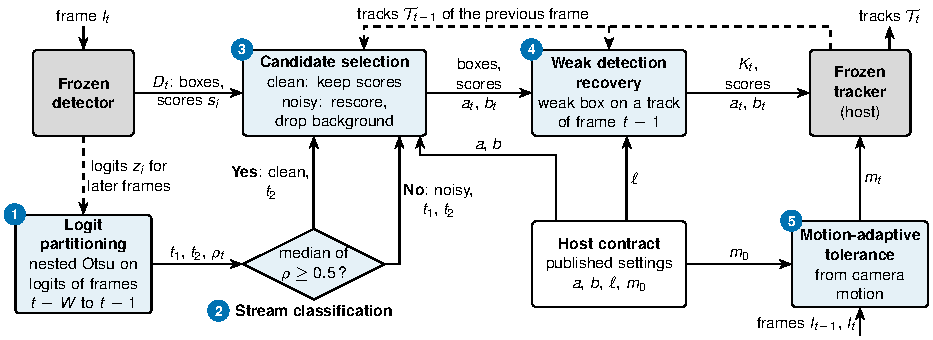
\includegraphics{Fig1.pdf}
\caption{\scl{} between a frozen detector and a frozen tracker (the host), for frame $t$. Each
arrow is labelled with the data it carries; dashed arrows carry data kept from earlier frames.
The diamond (Step 2) is a decision: the stream is clean (Yes) if the median of $\rho$ is at least
0.5, and noisy (No) otherwise. Steps 1--5 are described in Sects.~\ref{sec:calib}--\ref{sec:motion}, and the host contract in
Sect.~\ref{sec:contract}; every symbol is explained in Table~\ref{tab:symbols}}
\label{fig:arch}
\end{figure*}

\emph{Score calibration and adaptive inference.} Detector families such as YOLOX, YOLOv8, and RT-DETR give different score distributions,
and calibration methods learn a mapping from labelled data \cite{kuppers2020detcalib}. Otsu's
method picks, without labels, the threshold that best splits a histogram into two groups
\cite{otsu1979}; \scl{} applies it to the logits of recent scores. Dynamic networks learn their
settings for each model \cite{han2022dynamic}, and our earlier controller, AC-MOT (submitted), sets the detector operating point from
image and track cues. \scl{} instead reads the scores and acts on the tracker's input and
thresholds.
% --- sections/03_method
\section{Proposed SCL Framework}\label{sec:method}

\scl{} is a lightweight, rule-based layer operating between a frozen detector and tracker (the
host) without modifying their underlying algorithms. Fig.~\ref{fig:arch} illustrates the five
processing steps of \scl{} for frame $t$. First, Otsu-based logit partitioning (Step~1) divides
recent detection scores into background, uncertain, and confident groups. Next, detection stream
classification (Step~2) determines whether the score distribution is clean or noisy based on
historical confidence statistics. Mode-adaptive candidate selection (Step~3) then retains,
removes, or remaps detection scores and adjusts the tracker's confidence thresholds according to
the operating mode. Track-guided weak detection recovery (Step~4) allows eligible low-confidence
detections to support track continuity. Finally, camera motion-adaptive matching tolerance
(Step~5) adjusts the association criterion according to estimated camera motion. The host
contract provides the tracker's published parameters, while the tracker performs its original
association and track-management operations unchanged.

Table~\ref{tab:symbols} lists every symbol of this section in plain words, with its value in a
real example, the clean stream of Fig.~\ref{fig:groups}a; the subsections below use the same
example, so each number can be followed from the input to the output.

% --- tables/tab_symbols
\begin{table}[!tb]
\caption{The symbols of Sect.~\ref{sec:method} in plain words. Example: the value in the clean
stream of Fig.~\ref{fig:groups}a (MOT17-02, frame 101, ByteTrack in its official setting), as
recorded by the frozen \scl{}; values marked e.g.\ are worked examples from the text.}
\label{tab:symbols}
\centering\footnotesize
\setlength{\tabcolsep}{3pt}
\begin{tabular}{@{}l>{\raggedright\arraybackslash}p{37mm}>{\raggedright\arraybackslash}p{22mm}@{}}
\toprule
Symbol & Meaning & Example\\
\midrule
$s_i$ & detector score of candidate $i$, between 0 and 1 & e.g.\ 0.9\\
$z_i$ & its logit, $\log\bigl(s_i/(1-s_i)\bigr)$, Eq.~\eqref{eq:logit} & e.g.\ $\log 9=2.2$\\
$W$ & number of past frames whose logits are pooled & 10\\
$Z_t^W$ & the logits of frames $t-W$ to $t-1$ & 916 logits\\
$t_1$ & first split: background lies below it & $-0.78$ (score 0.32)\\
$t_2$ & second split: confident lies above it & 0.95 (score 0.72)\\
$\rho_t$ & share of confident candidates in the foreground, Eq.~\eqref{eq:rho} & $175/263=0.67$\\
median $\rho$ & median of $\rho$ over the stream so far; clean if $\ge0.5$ & 0.63: clean\\
$a$, $b$ & the tracker's published scores to match a track and to start one & 0.6, 0.7\\
$\ell$ & the lowest score the tracker uses & 0.1\\
$m_0$ & the tracker's matching tolerance: 1 minus the smallest IoU that matches & 0.8 (IoU $\ge0.2$)\\
$a_t$, $b_t$ & the thresholds \scl{} passes for frame $t$ & 0.6, 0.7 (kept)\\
$u_i$, $\tilde{s}_i$ & rank of $s_i$ among stored scores, and the new score of the noisy mode, Eq.~\eqref{eq:remap} & e.g.\ $u_i=0.8\to\tilde{s}_i=0.9$\\
$\mathcal{T}_{t-1}$ & the tracks of the previous frame & --\\
$K_t$ & the candidates passed to the tracker & --\\
$g_t$, $r_t$ & camera shift between two frames; its ratio to the usual shift & e.g.\ $r_t=2$\\
$m_t$ & the tolerance \scl{} passes for frame $t$, Eq.~\eqref{eq:motion} & 0.8 (clean)\\
\bottomrule
\end{tabular}
\end{table}


\subsection{Inputs and outputs of SCL}\label{sec:problem}
In each frame $t$, the detector gives candidates $D_t=\{(\mathbf{x}_i,s_i,c_i)\}$, each with a box
$\mathbf{x}_i$, a score $s_i\in(0,1)$, and a class $c_i$. The layer works on the logit
\begin{equation}
z_i=\log\frac{s_i}{1-s_i},
\label{eq:logit}
\end{equation}
the log-odds transformation of the confidence score. It maps a score between 0 and 1 to an
unbounded scale and keeps the order of the scores: a score of 0.5 gives $z_i=\log1=0$, 0.9 gives
$\log(0.9/0.1)=\log9=2.2$, and 0.1 gives $\log(1/9)=-2.2$. The logistic function $\sigma(z)=1/(1+e^{-z})$ turns a logit back into a
score. The layer uses logits for two reasons. Detector scores crowd near 0 and 1, where small
differences in score are large differences in confidence; the logit spreads these regions out, so
the splits of Step~1 separate the groups more clearly. And a common change of a detector's scores,
a change of temperature, divides all logits by the same number; the splits follow this stretch,
and each group keeps the same candidates. The host gives its contract $h=(a,b,\ell,m_0)$: the score $a$ needed to match a track, the
score $b$ needed to start one, the lowest score $\ell$ it uses, and its matching tolerance $m_0$,
one minus the smallest intersection over union (IoU) of two boxes that counts as a match. A
single-stage tracker has $\ell=\min(a,b)$, a two-stage tracker $\ell<\min(a,b)$. Table~\ref{tab:contracts}
(Sect.~\ref{sec:contract}) gives these four values for every tracker and the published settings they
come from; for ByteTrack in its official setting they are $a=0.6$, $b=0.7$, $\ell=0.1$, and
$m_0=0.8$. In every frame
the layer returns
\begin{equation}
\left(K_t,\tilde{s},a_t,b_t,m_t\right)=
\mathcal{L}\left(Z_{<t},D_t,\mathcal{T}_{t-1},g_t;\,h\right):
\label{eq:layer}
\end{equation}
the candidates $K_t$ for the tracker, their scores, and its thresholds and tolerance (the arrows
into the tracker in Fig.~\ref{fig:arch}), from the logits $Z_{<t}$ of earlier frames, the tracks
$\mathcal{T}_{t-1}$, and the camera motion $g_t$ between the frames $I_{t-1}$ and $I_t$; no future
frame is used.

% --- tables/tab1_contracts
\begin{table*}[!t]
\caption{Host contracts: the four published settings of each tracker that \scl{} reads, and where
each value comes from. $a$: the score a detection needs to be matched to a track; $b$: the score it
needs to start a new track; $\ell$: the lowest score the tracker uses at all; $m_0$: the matching
tolerance, one minus the smallest overlap (IoU) that counts as a match. A tracker with a second
step for low scores (two-stage) has $\ell<\min(a,b)$; a tracker without it (single-stage) has
$\ell=\min(a,b)$. ByteTrack-type trackers publish $m_0$ directly (match\_thresh); SORT-type
trackers publish the IoU threshold $\theta$, and $m_0=1-\theta$.}
\label{tab:contracts}
\centering\footnotesize
\setlength{\tabcolsep}{4pt}
\begin{tabular}{@{}>{\raggedright\arraybackslash}p{30mm}lcccc>{\raggedright\arraybackslash}p{78mm}@{}}
\toprule
Tracker (setting) & Type & $a$ & $b$ & $\ell$ & $m_0$ & Published settings behind the values\\
\midrule
ByteTrack (official MOT17) & two-stage & 0.6 & 0.7 & 0.1 & 0.8 & track\_thresh 0.6; new tracks need track\_thresh $+$ 0.1; second step from 0.1; match\_thresh 0.8\\
ByteTrack (library default) & two-stage & 0.25 & 0.25 & 0.1 & 0.8 & Ultralytics bytetrack.yaml: track\_high\_thresh 0.25, new\_track\_thresh 0.25, track\_low\_thresh 0.1, match\_thresh 0.8\\
BoT-SORT (library default) & two-stage & 0.25 & 0.25 & 0.1 & 0.8 & Ultralytics botsort.yaml: the same four values\\
SparseTrack & two-stage & 0.6 & 0.7 & 0.1 & 0.85 & track\_thresh 0.6; new tracks need track\_thresh $+$ 0.1; second step from 0.1; match\_thresh 0.85\\
BoostTrack & two-stage & 0.6 & 0.6 & 0.1 & 0.7 & det\_thresh 0.6; every emitted detection (from 0.1) can be boosted; IoU threshold 0.3\\
Hybrid-SORT & two-stage & 0.6 & 0.6 & 0.1 & 0.75 & det\_thresh 0.6; low-score step from 0.1; IoU threshold 0.25\\
OC-SORT & single-stage & 0.6 & 0.6 & 0.6 & 0.7 & det\_thresh 0.6, no low-score step; IoU threshold 0.3\\
PD-SORT & single-stage & 0.6 & 0.6 & 0.6 & 0.7 & det\_thresh 0.6, no low-score step; IoU threshold 0.3\\
\bottomrule
\end{tabular}
\end{table*}

\subsection{Otsu-Based Logit Partitioning and Confidence Estimation}\label{sec:calib}
\emph{Step 1 in Fig.~\ref{fig:arch}. Input:} the logits $Z_t^W$ of the candidates of the last $W=10$ frames. \emph{Output:} the
splits $t_1$, $t_2$ and the confident share $\rho_t$.

The logits are split twice with Otsu's method \cite{otsu1979}, which picks, from the data alone
and without labels or tuning, the threshold that best separates a set of values into two groups;
applied twice, it gives the three groups that one threshold cannot. The first split, $t_1$,
separates background (low logits) from foreground; the second, $t_2$, found on the foreground only,
divides it into uncertain and confident candidates. The share of confident candidates in the
foreground,
\begin{equation}
\rho_t=\frac{\left|\{z\in Z_t^W: z\ge t_2\}\right|}{\left|\{z\in Z_t^W: z\ge t_1\}\right|},
\label{eq:rho}
\end{equation}
describes the shape of the score distribution. For example, for the scores
0.02, 0.03, 0.05, 0.4, 0.5, 0.9, and 0.95 (logits $-3.9$, $-3.5$, $-2.9$, $-0.4$, 0, 2.2, and 2.9),
Otsu's method puts the first split at $t_1=-1.67$ (score 0.16), so the three lowest scores are
background, and the second at $t_2=1.10$ (score 0.75), so 0.4 and 0.5 are uncertain and 0.9 and
0.95 confident; two of the four foreground scores are confident, so $\rho_t=2/4=0.5$.
Fig.~\ref{fig:groups} shows the same for real streams. In the clean stream of
Fig.~\ref{fig:groups}a, the window holds 916 candidates: 653 lie below $t_1=-0.78$ (score 0.32),
88 between the splits, and 175 above $t_2=0.95$ (score 0.72), so $\rho_t=175/(88+175)=0.67$. In
the noisy stream of Fig.~\ref{fig:groups}b, 1,037 are background, 99 uncertain, and 83 confident,
so $\rho_t=83/(99+83)=0.46$. When a detector emits very few low scores, the first split falls inside
the objects; since clutter usually gives more candidates than the objects do, a window with fewer
candidates below $t_1$ than above it counts as clean, $\rho_t=1$ (background check). In both
streams of Fig.~\ref{fig:groups}, the background is larger than the foreground (653 against 263,
and 1,037 against 182), so the check does not apply.

\begin{figure}[t]
\centering
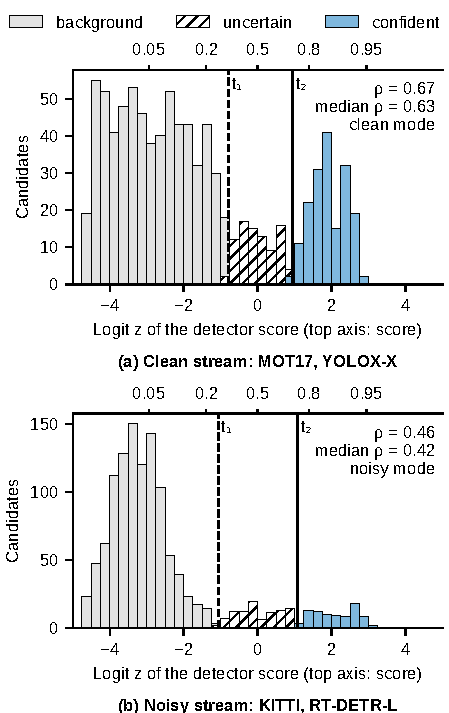
\includegraphics{Fig2.pdf}
\caption{What \scl{} sees just before its decision for frame 101: a histogram of the candidates
of the last 10 frames. Bottom axis: the logit of the detector score; top axis: the same position as
a score; height: the number of candidates. Dashed line: first split $t_1$; solid line: second split
$t_2$. Light gray bars: background (below $t_1$); hatched bars: uncertain (between the splits);
blue bars: confident (above $t_2$). $\rho$: the share of confident candidates in the foreground; the
median of $\rho$ decides the mode. (a) MOT17 sequence MOT17-02, published YOLOX-X detections, ByteTrack in its
official setting: $\rho=175/263=0.67$ and median $\rho=0.63\ge0.5$, so the stream is clean. (b)
KITTI sequence 0001, RT-DETR-L, ByteTrack in its library setting: $\rho=83/182=0.46$ and median $\rho=0.42<0.5$,
so the stream is noisy. All values were recorded by the frozen \scl{} in the runs of
Sect.~\ref{sec:results}}
\label{fig:groups}
\end{figure}

\subsection{Median-Based Detection Stream Classification}\label{sec:regimes}
\emph{Step 2 in Fig.~\ref{fig:arch}. Input:} the values $\rho$ of all frames so far. \emph{Output:} the mode of frame $t$.

The mode describes the distribution of the scores, not whether a single detection is correct. The
stream is clean at frame $t$ if the median of all $\rho$ values so far is at least one half, a
majority rule, and noisy otherwise; before the first valid split it is cold. In
Fig.~\ref{fig:groups}a, the first frame has no past frames and is cold, and frames 2 to 101 give 100
values of $\rho$ whose median is 0.63, so frame 101 is clean; in Fig.~\ref{fig:groups}b the median of
the same 100 frames is 0.42, so it is noisy.

\emph{Mode stability and adaptation delay.} The whole-stream median trades speed for stability. A
short run of low scores, such as a few frames of blur or occlusion, cannot change the mode, so the
layer does not switch modes in the middle of a stream; during development this rule raised the
HOTA of ByteTrack and OC-SORT (Sect.~\ref{sec:steps}). The cost is a delay after a lasting change
of the detector within one stream: a stream that was clean for $N$ frames turns noisy only after
more than $N$ noisy frames, because only then do they form the majority of the $\rho$ values. Two
parts of the layer do not wait. The splits use only the last $W$ frames, so the groups, and in
the clean mode the thresholds of Step~3, follow a new score scale within $W$ frames, and the
recovery of Step~4 works in both modes; only the rescoring of the noisy mode waits for the mode. A
median over the last $K$ frames bounds the delay to about $K/2$ frames;
Sect.~\ref{sec:ablation} tests $K=100$ and $K=300$.

\subsection{Mode-Adaptive Detection Candidate Selection and Threshold Adjustment}\label{sec:choice}
\emph{Step 3 in Fig.~\ref{fig:arch}. Input:} $D_t$, the mode, $t_1$, $t_2$, the thresholds $a$, $b$, and the tracks
$\mathcal{T}_{t-1}$. \emph{Output:} the kept boxes, their scores, and the thresholds $a_t$, $b_t$.

\emph{Cold and clean modes.} The tracker keeps its own thresholds and scores, and only cross-class
duplicates are removed. In the clean mode, a threshold so high that it would reject the confident
group is lowered to the score $\sigma(t_2)$ at which that group begins:
\begin{equation}
a_t=\min\!\left(a,\sigma(t_2)\right),\qquad b_t=\min\!\left(b,\sigma(t_2)\right).
\label{eq:clean}
\end{equation}
In Fig.~\ref{fig:groups}a, $\sigma(t_2)=0.72$ is above both $a=0.6$ and $b=0.7$, so
$a_t=\min(0.6,0.72)=0.6$ and $b_t=\min(0.7,0.72)=0.7$: the published thresholds are kept. The clean
mode is thus a minimal intervention rather than a plain pass-through: the scores are
kept, and the output equals that of the host alone whenever the confident group lies above the
host's thresholds and no rescue applies, as for BoostTrack, ByteTrack at floor 0.1, and Hybrid-SORT
on MOT17 (Sect.~\ref{sec:results}). When the scores are halved, for example, no score is above 0.5,
and ByteTrack in its official setting ($a=0.6$, $b=0.7$) never starts a track; the splits move with
the halved scores, so $\sigma(t_2)$ falls below 0.5, Eq.~\eqref{eq:clean} lowers both thresholds to
it, and the confident candidates reach the tracker again.

\emph{Noisy mode.} Background candidates ($z<t_1$) are dropped. Each remaining score is
replaced by its mid-rank $u_i\in(0,1)$ among the scores of a remap memory: the share of the stored
scores that are lower than $s_i$, with equal scores counted half. The memory stores the scores
kept in the first frame and in every 10th frame, the last 20 of them (before the first sample the
current frame is used). The new score is
\begin{equation}
\tilde{s}_i=
\begin{cases}
0.5+0.5\,u_i, & z_i\ge t_2,\\
0.1+0.4\,u_i, & t_1\le z_i<t_2,
\end{cases}
\label{eq:remap}
\end{equation}
and both thresholds are set to $a_t=b_t=0.5$. For example, a confident candidate whose score is
higher than 80\% of the stored scores ($u_i=0.8$) gets $0.5+0.5\cdot0.8=0.9$, and an uncertain one
with $u_i=0.3$ gets $0.1+0.4\cdot0.3=0.22$. Confident candidates ($z\ge t_2$) then get scores above 0.5
and may start and continue tracks, and uncertain ones ($t_1\le z<t_2$) get scores below 0.5 and may
only continue tracks through a tracker's low-score step. A weaker
candidate that overlaps a stronger one with IoU above one half is removed, unless a different track
of the previous frame claims it, which keeps people who stand close together in a crowd.

\emph{Score remapping is not probability calibration.} Formal calibration learns, from labelled
data, a map from a score to the probability that the detection is correct \cite{kuppers2020detcalib}.
The remap of Eq.~\eqref{eq:remap} needs no labels and estimates no probability. It keeps the order
of the scores within each group and places the groups in fixed ranges, so that the tracker's own
thresholds read the decision of the layer: a score above 0.5 means ``may start a track'', a score
between 0.1 and 0.5 ``may only continue one''. A remapped score of 0.8 therefore says that the
candidate ranks high among recent confident candidates, not that it is correct with probability
0.8. Because only ranks are used, the remap itself is unchanged by any order-preserving change of
the detector's scores, whereas a learned calibration map would have to be learned again.

\subsection{Track-Guided Weak Detection Recovery}\label{sec:rescue}
\emph{Step 4 in Fig.~\ref{fig:arch}. Input:} the output of Step~3, the tracks $\mathcal{T}_{t-1}$, and $\ell$. \emph{Output:}
$K_t$, their scores, and $a_t$, $b_t$ for the tracker.

A track can be lost when its object gets low scores for a few frames, above all in single-stage
trackers, which have no low-score step. The rescue passes such a candidate, with its score raised
just above the lowest threshold of the frame ($\ell$ for a two-stage tracker, the lower of $a_t$
and $b_t$ for a single-stage one), when it is in the foreground (or, for a single-stage tracker,
when there is no background group), overlaps a track of the previous frame with IoU of at least
one half, no other usable candidate covers that track, and the tracker could not see it otherwise.
For example, for ByteTrack in its official setting (two-stage, $\ell=0.1$) a rescued candidate gets
$0.1+0.001=0.101$ and enters its low-score step; for OC-SORT in a noisy frame (single-stage,
$a_t=b_t=0.5$) it gets $0.501$. It thus gives single-stage trackers the continuation step they
lack. The rescue only makes the box
visible; the tracker itself still decides, with its own matching, whether and to which track it is
assigned.

\subsection{Camera Motion-Adaptive Matching Tolerance}\label{sec:motion}
\emph{Step 5 in Fig.~\ref{fig:arch}. Input:} the frames $I_{t-1}$, $I_t$ and the tolerance $m_0$. \emph{Output:} the tolerance
$m_t$ of frame $t$.

In noisy frames, the matching tolerance grows with camera motion, because fast motion moves boxes
far from their tracks; otherwise $m_t=m_0$. The motion $g_t$ is the shift between consecutive
grayscale frames at quarter resolution, found by phase correlation \cite{reddy1996phasecorr}, and
$r_t$ is its ratio to its median over the last 100 frames ($r_t=1$ during a warm-up of 5 frames or
if this median is zero):
\begin{equation}
m_t=\min\!\left(0.95,\;1-\frac{1-m_0}{\max(1,r_t)}\right).
\label{eq:motion}
\end{equation}
For example, with $m_0=0.8$ a match needs an IoU of at least $1-0.8=0.2$. If, in a noisy frame,
the camera moves twice as much as usual ($r_t=2$), then $m_t=\min(0.95,\,1-0.2/2)=0.9$, and a match
needs an IoU of only 0.1. The cap 0.95 keeps a smallest overlap of 0.05.

\subsection{SCL Integration with Existing Trackers}\label{sec:contract}
Table~\ref{tab:contracts} lists the contracts; each value is taken from the tracker's published
configuration, and none is fitted. For each tracker family, a small adapter links the layer to the
tracker block of Fig.~\ref{fig:arch}: it writes the layer's candidates, scores, thresholds, and
tolerance into the tracker's existing parameters before each update and then calls the tracker's
own update. The matching steps, motion model, track management, and any post-processing of the
authors run unchanged, so the host stays frozen: only the values of its thresholds are set for
each frame, and the rules are the same for every tracker.


\begin{table}[!tb]
\caption{The fixed values of \scl{}: each row gives one value, its setting, and where it comes from: a standard value of MOT evaluation, a common threshold, a definition, or a design choice made once at the start of development and never tuned. The same values are used for every tracker, detector, and dataset.}
\label{tab:constants}
\centering\footnotesize
\setlength{\tabcolsep}{3pt}
\begin{tabular}{@{}>{\raggedright\arraybackslash}p{19mm}>{\raggedright\arraybackslash}p{27mm}>{\raggedright\arraybackslash}p{25mm}@{}}
\toprule
Value & Setting & Source\\
\midrule
Window $W$ & 10 frames & design choice\\
Mode rule & clean if median $\rho\ge0.5$ & majority rule\\
Background check & $\rho=1$ if fewer below $t_1$ than above & rule: no background group\\
Noisy score ranges & $[0.5,1)$, $[0.1,0.5)$ & common thresholds\\
Noisy $a_t$, $b_t$ & 0.5 & common threshold\\
Remap memory & 20 frames, one every 10 & design choice\\
Duplicate, rescue IoU & 0.5 & MOT evaluation IoU\\
Rescued score & lowest threshold $+\,0.001$ & just above the threshold\\
Motion cue & phase correlation, quarter resolution & standard method \cite{reddy1996phasecorr}\\
Motion history & 100 frames, warm-up 5 & design choice\\
Tolerance cap & 0.95 & minimum overlap 0.05\\
\bottomrule
\end{tabular}
\end{table}

\subsection{Fixed SCL Parameters}\label{sec:constants}
Table~\ref{tab:constants} lists all values of \scl{}. They were fixed before the external
evaluation, are the same for every tracker, detector, and dataset, and none was chosen by searching
over a range of values. They come from standard values (the IoU of 0.5 of MOT evaluation and the
common thresholds 0.5 and 0.1), from definitions, and from design choices kept fixed in all
development stages. Algorithm~\ref{alg:layer} gives Steps 1--5 for one frame.

\begin{algorithm}[t]
\caption{\scl{} for frame $t$; the comments name the steps of Fig.~\ref{fig:arch}. The window
holds the logits of frames $t-W$ to $t-1$, so the decision for frame $t$ uses no future frame.}\label{alg:layer}
\begin{algorithmic}[1]
\Require candidates $D_t$, tracks $\mathcal{T}_{t-1}$, motion cue $g_t$, contract $(a,b,\ell,m_0)$, constants of Table~\ref{tab:constants}
\Ensure candidates $K_t$, scores $\tilde{s}$, thresholds $a_t,b_t$, tolerance $m_t$
\State $z_i\gets$ logit of $s_i$ for all $i$ \Comment{Eq.~\eqref{eq:logit}}
\If{no valid split exists} \Comment{e.g., first frame}
  \State mode $\gets$ cold; $(a_t,b_t)\gets(a,b)$
\Else
  \State $(t_1,t_2)\gets$ nested Otsu on the window \Comment{Step 1}
  \State $\rho_t\gets$ Eq.~\eqref{eq:rho} with the background check
  \State mode $\gets$ clean if $\mathrm{median}(\rho)\ge0.5$, else noisy \Comment{Step 2}
\EndIf
\If{mode is cold or clean} \Comment{Step 3}
  \State remove cross-class duplicates; keep raw scores
  \If{clean} set $(a_t,b_t)$ by Eq.~\eqref{eq:clean}
  \EndIf
\Else \Comment{noisy mode}
  \State remove duplicates with track context
  \State drop $z<t_1$; remap scores by Eq.~\eqref{eq:remap}
  \State $a_t\gets0.5$; $b_t\gets0.5$
\EndIf
\State rescue continuations (not cold) \Comment{Step 4}
\State $m_t\gets$ Eq.~\eqref{eq:motion} if noisy, else $m_0$ \Comment{Step 5}
\State pass $K_t$, $\tilde{s}$, $a_t$, $b_t$, $m_t$ to the tracker
\State add the logits left after duplicate removal to the window
\State add $g_t$ to the motion history
\State store the tracks of frame $t$ after the tracker update
\end{algorithmic}
\end{algorithm}
% --- sections/04_development
\section{SCL Development and Refinement}\label{sec:development}

This section presents the development and refinement of \scl{} using the development data
described in Sect.~\ref{sec:data}. Section~\ref{sec:prior} introduces the initial always-on banding
(\aob{}) design and discusses its limitations. Section~\ref{sec:steps} describes the incremental
improvements that addressed these limitations, supported by the experimental comparisons in
Table~\ref{tab:ablation}. Finally, Sect.~\ref{sec:freeze} explains the configuration freezing and
validation procedures performed before external evaluation to ensure reproducibility and prevent
changes based on subsequent results.

% --- tables/tab6_ablation
\begin{table*}[!tp]
\caption{How \scl{} was built from \aob{} on development data. Upper part: each row adds one change to the row above; Effect gives the HOTA (\%) before and after that change (``A to B'') or compared with the tracker alone (host). The number in parentheses after ByteTrack and OC-SORT is the lowest emitted detector score. Lower part: versions that were tested and not kept, with the reason.}
\label{tab:ablation}
\centering\footnotesize
\setlength{\tabcolsep}{4pt}
\begin{tabular}{@{}>{\raggedright\arraybackslash}p{25mm}>{\raggedright\arraybackslash}p{36mm}>{\raggedright\arraybackslash}p{62mm}@{}}
\toprule
Step & Change & Effect\\
\midrule
\aob{} emulated & always-noisy bands, overlap deduplication, rank remap & ByteTrack (0.1) 56.41 vs host 67.70; OC-SORT (0.1) 45.72 vs 66.44\\
+ mode gate & mode statistic, host-anchored clean mode, crowd-safe duplicates & SparseTrack 64.72 to 68.93 (host 68.88); BoostTrack 62.61 to 68.37 (host 68.49)\\
+ whole-stream mode & mode from all past frames & ByteTrack (0.1) 67.561 to 67.702; OC-SORT (0.1) 65.697 to 66.071\\
+ continuation rescue & foreground track-consistent rescue & OC-SORT (0.01) 66.405 to 66.619; OC-SORT (0.1) 66.071 to 66.469\\
+ background check = \scl{} & no background mode gives no evidence against the host & ByteTrack/BoostTrack (0.1) identical to host; OC-SORT 67.041 (0.01), 66.907 (0.1)\\
\midrule
\multicolumn{2}{@{}l}{\textit{Rejected version}} & \textit{Evidence}\\
\multicolumn{2}{@{}l}{no candidates at frame 1} & $-0.3$ to $-0.5$ HOTA on every MOT17 host\\
\multicolumn{2}{@{}l}{rescue below a two-stage host's low stage} & FP $+700$ to $+1000$, $-0.4$ to $-0.5$ HOTA\\
\multicolumn{2}{@{}l}{rank-remapped scores in clean frames} & ByteTrack $-0.2$ / $-1.6$ HOTA\\
\multicolumn{2}{@{}l}{host-clipped noisy primary band} & KITTI YOLOv8n ByteTrack $+1.4$ HOTA but uncontrolled false tracks on a noisy aerial stream (26.9 vs 14.9 boxes/frame)\\
\bottomrule
\end{tabular}
\end{table*}
% --- tables/tab_prior
\begin{table*}[!t]
\caption{MOT17 val-half with the published YOLOX-X detections: the earlier design \aob{} and the final \scl{}, each added to the same strong tracker. Host: the tracker alone; Host+\aob{} and Host+\scl{}: the same tracker with each layer, on the same detections. Change: the run with the layer minus Host, with its 95\% bootstrap interval in brackets; a negative HOTA, MOTA, or IDF1 change means the layer made the tracker worse; bold: the interval does not include zero, so the change is reliable. $\uparrow$: higher is better; $\downarrow$: lower is better (IDS: identity switches, a count).}
\label{tab:prior}
\centering\footnotesize
\setlength{\tabcolsep}{6pt}
\begin{tabular}{@{}lrrlrl@{}}
\toprule
Metric & Host & Host+\aob{} & \aob{} change [95\% CI] & Host+\scl{} & \scl{} change [95\% CI]\\
\midrule
\multicolumn{6}{@{}l}{\textit{SparseTrack} \cite{liu2025sparsetrack}}\\
\quad HOTA$\uparrow$ & 68.88 & 64.72 & {\boldmath $-4.15$ [$-5.54$, $-1.66$]} & 68.93 & $+0.06$ [$-0.01$, $+0.25$]\\
\quad MOTA$\uparrow$ & 77.85 & 71.71 & {\boldmath $-6.14$ [$-8.10$, $-2.74$]} & 77.93 & $+0.08$ [$-0.03$, $+0.30$]\\
\quad IDF1$\uparrow$ & 81.97 & 77.49 & {\boldmath $-4.49$ [$-6.19$, $-1.96$]} & 82.13 & $+0.16$ [$-0.02$, $+0.70$]\\
\quad IDS$\downarrow$ & 124 & 108 & $-16$ [$-47$, $+12$] & 131 & $+7$ [$0$, $+19$]\\
\multicolumn{6}{@{}l}{\textit{BoostTrack, online} \cite{stanojevic2024boosttrack}}\\
\quad HOTA$\uparrow$ & 68.49 & 62.61 & {\boldmath $-5.89$ [$-7.76$, $-2.87$]} & 68.49 & 0 (identical)\\
\quad MOTA$\uparrow$ & 75.50 & 66.64 & {\boldmath $-8.87$ [$-12.37$, $-7.14$]} & 75.50 & 0 (identical)\\
\quad IDF1$\uparrow$ & 81.41 & 75.19 & {\boldmath $-6.22$ [$-9.33$, $-2.85$]} & 81.41 & 0 (identical)\\
\quad IDS$\downarrow$ & 113 & 75 & {\boldmath $-38$ [$-81$, $-1$]} & 113 & 0 (identical)\\
\multicolumn{6}{@{}l}{\textit{BoostTrack, with GBI} \cite{stanojevic2024boosttrack}}\\
\quad HOTA$\uparrow$ & 71.73 & 66.35 & {\boldmath $-5.37$ [$-7.30$, $-2.75$]} & 71.73 & 0 (identical)\\
\quad MOTA$\uparrow$ & 81.03 & 72.30 & {\boldmath $-8.73$ [$-12.59$, $-6.50$]} & 81.03 & 0 (identical)\\
\quad IDF1$\uparrow$ & 84.16 & 78.51 & {\boldmath $-5.65$ [$-8.96$, $-2.77$]} & 84.16 & 0 (identical)\\
\quad IDS$\downarrow$ & 97 & 70 & $-27$ [$-73$, $+11$] & 97 & 0 (identical)\\
\bottomrule
\end{tabular}
\end{table*}
\subsection{Initial Design and Limitations}\label{sec:prior}
The earlier design \aob{} computed the same nested Otsu groups but treated every stream as noisy:
in every frame it applied the groups, removed every weaker candidate that overlapped a stronger one
with IoU above one half, and rescored all candidates by rank. Table~\ref{tab:prior} compares \aob{}
and \scl{} with strong published trackers on MOT17. \aob{} lowered the HOTA of SparseTrack by 4.15
points and of BoostTrack by 5.89 points online and 5.37 points with its gap-filling post-processing
(GBI), for two reasons: removing overlapping boxes deleted people hidden behind others in crowds,
and its thresholds were stricter than the trackers' own. With the same trackers, \scl{} changed
HOTA by $+0.06$ for SparseTrack and left both BoostTrack versions identical to the host. A layer
that acts in every frame therefore cannot be placed safely in front of an unknown tracker, and the
next steps let the layer decide from the scores whether to act at all.


\subsection{Incremental Design Improvements}\label{sec:steps}
Each step was compared with the step before it (Table~\ref{tab:ablation}). The \emph{mode gate}
added the mode check, the clean mode that keeps the tracker's scores and thresholds, and the crowd-safe duplicate
rule; it restored SparseTrack from 64.72 to 68.93 HOTA and BoostTrack from 62.61 to 68.37. The
\emph{whole-stream mode} removed mode changes in the middle of streams and raised ByteTrack from
67.561 to 67.702 and OC-SORT from 65.697 to 66.071. The \emph{continuation rescue} added 0.2 to 0.4
points for OC-SORT. The \emph{background check} completed \scl{}: ByteTrack and BoostTrack returned
to output identical to the host, and OC-SORT rose to 67.04 and 66.91 at the two floors. Four other
variants were tested and not kept.


\subsection{Configuration Freezing and Validation}\label{sec:freeze}
The final configuration was frozen before any external test as a version-control tag, protected
by a lock file with a cryptographic hash of the layer, its configuration, and the evaluation
scripts. Sixty-one automated tests check, among others, that the layer uses no future data and
passes clean streams unchanged. All results of Sect.~\ref{sec:results} come from this frozen
configuration; the comparisons, the ablation, and the sensitivity analysis were run after the
freeze, through run-time options of the evaluation scripts, and changed none of its values.
% --- sections/05_results
\section{Experimental Results and Evaluation}\label{sec:results}

This section evaluates the effectiveness and generalization of \scl{} against the host trackers
using identical detections and published tracker configurations. Section~\ref{sec:tracker}
examines tracking performance across different trackers on MOT17, while Sect.~\ref{sec:detector}
evaluates detector--tracker compatibility on KITTI. Section~\ref{sec:shift} investigates robustness
to detection confidence-score shifts, and Sect.~\ref{sec:baselines} compares \scl{} with adaptive
thresholding methods. Section~\ref{sec:ablation} presents component ablation and parameter
sensitivity analyses. Finally, Sects.~\ref{sec:external} and~\ref{sec:visdrone} assess
generalization to previously unseen trackers and the held-out UAVDT dataset, respectively. In all
comparisons, the baseline is the host tracker operating without \scl{}, and Fig.~\ref{fig:forest}
summarizes the HOTA differences across the evaluated configurations.

\emph{How to read the result tables.} Each result table compares two runs on the same detections:
A, the tracker alone (Host), and B, the same tracker with \scl{} (Host+\scl{}). HOTA, MOTA, and
IDF1 are percentages, and higher is better ($\uparrow$); IDS counts identity switches, and lower is
better ($\downarrow$). The column Change gives B minus A, so a positive change in HOTA, MOTA, or
IDF1 and a negative change in IDS mean that \scl{} helped. The brackets give the 95\% bootstrap
interval of the change: when the whole interval lies on one side of zero, the change is reliable
and printed in bold; when it includes zero, A and B are not reliably different. ``Identical'' means
that \scl{} did not change the tracker's output at all. For example, in Table~\ref{tab:kitti}
ByteTrack with RT-DETR-L has a MOTA of 47.27 alone and 53.24 with \scl{}; the change is $+5.98$
points, and its interval $[+1.16,+9.94]$ lies above zero, so the gain is reliable. Values are
rounded separately, so B minus A can differ from the change in the last digit.

\begin{figure}[!t]
\centering
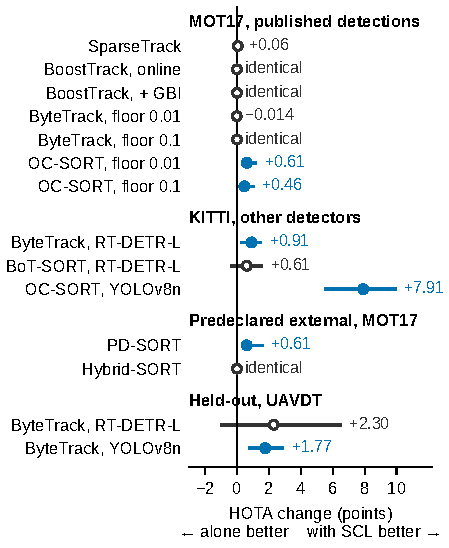
\includegraphics{Fig3.pdf}
\caption{Summary of all HOTA results: for every tested tracker and detector, how much \scl{}
changes HOTA (tracker with \scl{} minus tracker alone, in points). Dot and number: the change; line:
its 95\% bootstrap interval. Right of the vertical line at zero, \scl{} is better. Filled dot: a
reliable gain (the whole interval is above zero); open dot: no reliable change (the interval
includes zero) or identical output}
\label{fig:forest}
\end{figure}

\subsection{Performance Across Trackers on MOT17}\label{sec:tracker}
Table~\ref{tab:mot17} shows the development trackers on MOT17 val-half. The two-stage trackers with
well-matched detections stayed at the accuracy of their hosts: BoostTrack, online and with GBI, and
ByteTrack at floor 0.1 gave exactly the same output, and ByteTrack at floor 0.01 and SparseTrack
stayed within 0.06 HOTA points, the self-limiting clean mode. The single-stage OC-SORT improved at
both floors (HOTA from 66.43 to 67.04 and from 66.44 to 66.91, MOTA $+1.27$ and $+1.26$), with fewer identity switches and
higher HOTA on 7 of 7 sequences, through the continuation rescue.

% --- tables/tab3_mot17
\begin{table}[!tb]
\caption{MOT17 val-half with the published YOLOX-X detections: each development tracker alone and with \scl{}. Host: the tracker alone; Host+\scl{}: the same tracker with \scl{}, on the same detections. Change: Host+\scl{} minus Host, with its 95\% bootstrap interval in brackets; bold: the interval does not include zero, so the change is reliable. $\uparrow$: higher is better; $\downarrow$: lower is better (IDS: identity switches, a count). Paper: the number reported by the tracker's authors (--: not reported). Floor: the lowest detector score emitted.}
\label{tab:mot17}
\centering\footnotesize
\setlength{\tabcolsep}{2.5pt}
\begin{tabular}{@{}lrrrl@{}}
\toprule
Metric & Paper & Host & \begin{tabular}[b]{@{}r@{}}Host\\+\scl{}\end{tabular} & Change [95\% CI]\\
\midrule
\multicolumn{5}{@{}l}{\textit{SparseTrack} \cite{liu2025sparsetrack}}\\
\quad HOTA$\uparrow$ & 69.2 & 68.88 & 68.93 & $+0.06$ [$-0.01$, $+0.25$]\\
\quad MOTA$\uparrow$ & 76.8 & 77.85 & 77.93 & $+0.08$ [$-0.03$, $+0.30$]\\
\quad IDF1$\uparrow$ & 81.4 & 81.97 & 82.13 & $+0.16$ [$-0.02$, $+0.70$]\\
\quad IDS$\downarrow$ & -- & 124 & 131 & $+7$ [$0$, $+19$]\\
\multicolumn{5}{@{}l}{\textit{BoostTrack, online} \cite{stanojevic2024boosttrack}}\\
\quad HOTA$\uparrow$ & 68.37 & 68.49 & 68.49 & 0 (identical)\\
\quad MOTA$\uparrow$ & 75.56 & 75.50 & 75.50 & 0 (identical)\\
\quad IDF1$\uparrow$ & 81.35 & 81.41 & 81.41 & 0 (identical)\\
\quad IDS$\downarrow$ & 118 & 113 & 113 & 0 (identical)\\
\multicolumn{5}{@{}l}{\textit{BoostTrack, + GBI} \cite{stanojevic2024boosttrack}}\\
\quad HOTA$\uparrow$ & 71.33 & 71.73 & 71.73 & 0 (identical)\\
\quad MOTA$\uparrow$ & 80.55 & 81.03 & 81.03 & 0 (identical)\\
\quad IDF1$\uparrow$ & 83.84 & 84.16 & 84.16 & 0 (identical)\\
\quad IDS$\downarrow$ & 106 & 97 & 97 & 0 (identical)\\
\multicolumn{5}{@{}l}{\textit{ByteTrack, floor 0.01} \cite{zhang2022bytetrack}}\\
\quad HOTA$\uparrow$ & -- & 67.70 & 67.68 & $-0.014$ [$-0.058$, $+0.009$]\\
\quad MOTA$\uparrow$ & 76.6 & 77.60 & 77.66 & $+0.06$ [$-0.15$, $+0.34$]\\
\quad IDF1$\uparrow$ & 79.3 & 79.47 & 79.44 & $-0.031$ [$-0.135$, $+0.035$]\\
\quad IDS$\downarrow$ & -- & 214 & 218 & $+4$ [$-2$, $+13$]\\
\multicolumn{5}{@{}l}{\textit{ByteTrack, floor 0.1} \cite{zhang2022bytetrack}}\\
\quad HOTA$\uparrow$ & -- & 67.70 & 67.70 & 0 (identical)\\
\quad MOTA$\uparrow$ & 76.6 & 77.60 & 77.60 & 0 (identical)\\
\quad IDF1$\uparrow$ & 79.3 & 79.47 & 79.47 & 0 (identical)\\
\quad IDS$\downarrow$ & -- & 214 & 214 & 0 (identical)\\
\multicolumn{5}{@{}l}{\textit{OC-SORT, floor 0.01} \cite{cao2023ocsort}}\\
\quad HOTA$\uparrow$ & 66.5 & 66.43 & 67.04 & {\boldmath $+0.61$ [$+0.36$, $+1.24$]}\\
\quad MOTA$\uparrow$ & 74.9 & 74.67 & 75.94 & {\boldmath $+1.27$ [$+0.17$, $+3.01$]}\\
\quad IDF1$\uparrow$ & 77.7 & 78.05 & 78.71 & $+0.66$ [$-0.25$, $+1.60$]\\
\quad IDS$\downarrow$ & -- & 211 & 203 & {\boldmath $-8$ [$-15$, $-2$]}\\
\multicolumn{5}{@{}l}{\textit{OC-SORT, floor 0.1} \cite{cao2023ocsort}}\\
\quad HOTA$\uparrow$ & 66.5 & 66.44 & 66.91 & {\boldmath $+0.46$ [$+0.27$, $+1.09$]}\\
\quad MOTA$\uparrow$ & 74.9 & 74.67 & 75.93 & {\boldmath $+1.26$ [$+0.37$, $+3.34$]}\\
\quad IDF1$\uparrow$ & 77.7 & 78.05 & 78.33 & {\boldmath $+0.287$ [$+0.003$, $+0.838$]}\\
\quad IDS$\downarrow$ & -- & 213 & 199 & $-14$ [$-38$, $+6$]\\
\bottomrule
\end{tabular}
\end{table}

\subsection{Cross-Detector Evaluation on KITTI}\label{sec:detector}
\begin{figure*}[t]
\centering
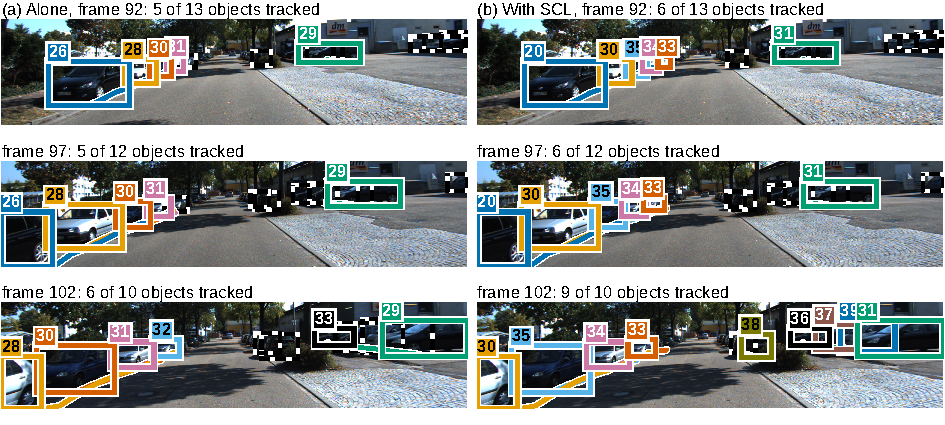
\includegraphics{Fig4.pdf}
\caption{The same video tracked twice: KITTI sequence 0001 \cite{geiger2012kitti} with OC-SORT
and YOLOv8n, at frames 92, 97, and 102 (rows). (a) The tracker alone; (b) the same tracker with
\scl{}. Each colour and number is one track (one object identity); its line shows where the object
was in the previous 20 frames. Dashed boxes: labelled objects that no track follows (missed). At
frame 102, the tracker alone follows 6 of the 10 labelled objects and with \scl{} 9. IDs are
numbered separately in each run. This sequence has the median HOTA gain of the 21 sequences, and frame 102 is its first frame with
the largest gain in tracked objects}
\label{fig:example}
\end{figure*}
Table~\ref{tab:kitti} shows what happens when the detector is replaced. With the noisy RT-DETR-L,
ByteTrack gained 5.98 MOTA, 3.87 IDF1, and 0.91 HOTA points, and BoT-SORT 7.86 MOTA, 3.10 IDF1,
and 0.61 HOTA points, with 297 and 226 fewer identity switches. With YOLOv8n, OC-SORT rose from 36.27 to 44.18
HOTA ($+7.91$ points, $[+5.47,+9.98]$), 9.40 MOTA points, and 9.60 IDF1 points; it followed many more objects, as
its missed objects (FN) fell by 5,310, and its identity switches rose with them by 79.
Fig.~\ref{fig:example} follows this cell over three frames: each object keeps its ID,
and at frame 102 OC-SORT alone tracked 6 of the 10 labelled objects and with \scl{} 9.

% --- tables/tab4_kitti
\begin{table}[!tb]
\caption{KITTI tracking training with detectors that the trackers were not tuned for (HOTA averaged over cars and pedestrians). Host: the tracker alone; Host+\scl{}: the same tracker with \scl{}, on the same detections. Change: Host+\scl{} minus Host, with its 95\% bootstrap interval in brackets; bold: the interval does not include zero, so the change is reliable. $\uparrow$: higher is better; $\downarrow$: lower is better (IDS: identity switches, a count). BoT-SORT: sequence 0020 is left out of both runs, because the BoT-SORT code stops with a numerical error on it.}
\label{tab:kitti}
\centering\footnotesize
\setlength{\tabcolsep}{2.5pt}
\begin{tabular}{@{}lrrl@{}}
\toprule
Metric & Host & \begin{tabular}[b]{@{}r@{}}Host\\+\scl{}\end{tabular} & Change [95\% CI]\\
\midrule
\multicolumn{4}{@{}l}{\textit{ByteTrack} \cite{zhang2022bytetrack}\textit{, RT-DETR-L}}\\
\quad HOTA$\uparrow$ & 50.73 & 51.64 & {\boldmath $+0.91$ [$+0.22$, $+1.55$]}\\
\quad MOTA$\uparrow$ & 47.27 & 53.24 & {\boldmath $+5.98$ [$+1.16$, $+9.94$]}\\
\quad IDF1$\uparrow$ & 64.98 & 68.86 & {\boldmath $+3.87$ [$+1.67$, $+5.06$]}\\
\quad IDS$\downarrow$ & 686 & 389 & {\boldmath $-297$ [$-530$, $-122$]}\\
\multicolumn{4}{@{}l}{\textit{BoT-SORT} \cite{aharon2022botsort}\textit{, RT-DETR-L} (20 sequences)}\\
\quad HOTA$\uparrow$ & 53.91 & 54.52 & $+0.61$ [$-0.39$, $+1.61$]\\
\quad MOTA$\uparrow$ & 48.25 & 56.11 & {\boldmath $+7.86$ [$+2.21$, $+13.44$]}\\
\quad IDF1$\uparrow$ & 67.74 & 70.85 & {\boldmath $+3.10$ [$+1.00$, $+4.57$]}\\
\quad IDS$\downarrow$ & 476 & 250 & {\boldmath $-226$ [$-369$, $-120$]}\\
\multicolumn{4}{@{}l}{\textit{OC-SORT} \cite{cao2023ocsort}\textit{, YOLOv8n}}\\
\quad HOTA$\uparrow$ & 36.27 & 44.18 & {\boldmath $+7.91$ [$+5.47$, $+9.98$]}\\
\quad MOTA$\uparrow$ & 33.99 & 43.39 & {\boldmath $+9.40$ [$+1.10$, $+12.30$]}\\
\quad IDF1$\uparrow$ & 50.46 & 60.05 & {\boldmath $+9.60$ [$+5.61$, $+12.16$]}\\
\quad IDS$\downarrow$ & 91 & 170 & {\boldmath $+79$ [$+43$, $+125$]}\\
\bottomrule
\end{tabular}
\end{table}
% --- tables/tab_shift
\begin{table}[!tb]
\caption{MOT17 val-half with the detector scores changed before the tracker, while the tracker keeps its published thresholds: $s^3$ cubes every score, $0.5\,s$ halves it, and $T=2$ and $T=0.5$ divide its logit by 2 or by 0.5. HOTA (\%, higher is better) of the tracker alone (Host) and with \scl{} (Host+\scl{}); 0.00 means that no object was tracked. Change: Host+\scl{} minus Host, with its 95\% bootstrap interval; bold: the interval does not include zero (a reliable change). Lowest emitted score 0.01 (BoostTrack 0.1).}
\label{tab:shift}
\centering\footnotesize
\setlength{\tabcolsep}{3pt}
\begin{tabular}{@{}lrrl@{}}
\toprule
 & \multicolumn{3}{c}{HOTA (\%)}\\
\cmidrule(l){2-4}
Score change & Host & \begin{tabular}[b]{@{}r@{}}Host\\+\scl{}\end{tabular} & Change [95\% CI]\\
\midrule
\multicolumn{4}{@{}l}{\textit{ByteTrack, official setting} \cite{zhang2022bytetrack}}\\
\quad $s^3$ & 60.92 & 65.81 & {\boldmath $+4.89$ [$+2.60$, $+13.69$]}\\
\quad $0.5\,s$ & 0.00 & 66.17 & {\boldmath $+66.17$ [$+49.32$, $+75.40$]}\\
\quad $T=2$ & 65.84 & 66.95 & {\boldmath $+1.11$ [$+0.35$, $+3.87$]}\\
\quad $T=0.5$ & 67.30 & 67.29 & $-0.009$ [$-0.051$, $+0.005$]\\
\multicolumn{4}{@{}l}{\textit{ByteTrack, library setting} \cite{zhang2022bytetrack}}\\
\quad $s^3$ & 66.31 & 66.31 & $-0.006$ [$-0.384$, $+0.383$]\\
\quad $0.5\,s$ & 66.61 & 66.48 & $-0.14$ [$-0.66$, $+0.14$]\\
\quad $T=2$ & 63.97 & 63.97 & 0 (identical)\\
\quad $T=0.5$ & 66.53 & 66.53 & $-0.006$ [$-0.029$, $+0.001$]\\
\multicolumn{4}{@{}l}{\textit{OC-SORT} \cite{cao2023ocsort}}\\
\quad $s^3$ & 58.34 & 66.60 & {\boldmath $+8.26$ [$+5.86$, $+16.81$]}\\
\quad $0.5\,s$ & 0.00 & 66.72 & {\boldmath $+66.72$ [$+50.32$, $+75.56$]}\\
\quad $T=2$ & 65.99 & 67.22 & {\boldmath $+1.24$ [$+0.52$, $+3.42$]}\\
\quad $T=0.5$ & 66.61 & 67.06 & $+0.45$ [$-0.01$, $+0.97$]\\
\multicolumn{4}{@{}l}{\textit{BoostTrack, online} \cite{stanojevic2024boosttrack}}\\
\quad $s^3$ & 61.33 & 64.84 & {\boldmath $+3.51$ [$+0.85$, $+13.28$]}\\
\quad $T=2$ & 67.59 & 67.59 & 0 (identical)\\
\bottomrule
\end{tabular}
\end{table}
% --- tables/tab_baselines
\begin{table}[!tb]
\caption{KITTI tracking training: HOTA (\%, higher is better) of the tracker alone (Host), of two simple adaptive baselines ($t_1$, $t_2$), and of \scl{}, on the same detections. In the baselines, the tracker's thresholds are set in every frame to the first ($t_1$) or second ($t_2$) Otsu split of the logits of the last 10 frames, and the scores are not changed. Halved: halved detector scores. \scl{} $-$ $t_2$: the gain of \scl{} over the stronger baseline, with its 95\% bootstrap interval below; bold: the interval does not include zero (a reliable gain).}
\label{tab:baselines}
\centering\footnotesize
\setlength{\tabcolsep}{3pt}
\begin{tabular}{@{}lrrrrc@{}}
\toprule
Cell & Host & $t_1$ & $t_2$ & \scl{} & \scl{} $-$ $t_2$\\
\midrule
\twol{OC-SORT,}{YOLOv8n} & 36.27 & 39.97 & 41.09 & 44.18 & \cib{+3.09}{+2.00}{+4.03}\\
\addlinespace[3pt]
\begin{tabular}[c]{@{}l@{}}ByteTrack,\\RT-DETR-L,\\halved\end{tabular} & 49.50 & 49.58 & 49.50 & 51.79 & \cib{+2.29}{+0.28}{+4.96}\\
\addlinespace[3pt]
\begin{tabular}[c]{@{}l@{}}OC-SORT,\\YOLOv8n,\\halved\end{tabular} & 0.00 & 37.68 & 43.56 & 46.30 & \cib{+2.74}{+1.32}{+3.34}\\
\bottomrule
\end{tabular}
\end{table}
% --- tables/tab_act
\begin{table*}[!tp]
\caption{ACT \cite{act2026adaptive} and \scl{} on the same detections and tracker. (a) HOTA in every tested setting. ACT, \scl{}: HOTA (\%, higher is better) of the tracker with each method. \scl{} $-$ ACT: how much higher \scl{} is than ACT in HOTA and in IDF1, with its 95\% bootstrap interval below. (b) MOTA and identity switches on UAVDT: the value with each method and \scl{} $-$ ACT with its 95\% bootstrap interval in brackets. A positive HOTA, IDF1, or MOTA difference and a negative IDS difference mean that \scl{} is better; bold: the interval does not include zero (a reliable difference). $\uparrow$: higher is better; $\downarrow$: lower is better (IDS: identity switches, a count). ACT uses its published parameters, without tuning. KITTI: HOTA averaged over cars and pedestrians; MOT17: val-half, the setting ACT was designed for; UAVDT: test split, one vehicle class, ignored regions removed (Sect.~\ref{sec:metrics}).}
\label{tab:act}
\centering\footnotesize
\setlength{\tabcolsep}{5pt}
{\textit{(a) HOTA and IDF1}}\par\smallskip
\begin{tabular}{@{}lllrrcc@{}}
\toprule
Data & Detector & Tracker & ACT & \scl{} & \scl{} $-$ ACT, HOTA & \scl{} $-$ ACT, IDF1\\
\midrule
KITTI, halved scores & RT-DETR-L & ByteTrack & 49.77 & 51.79 & \cib{+2.01}{+0.01}{+4.76} & \ci{+1.70}{-1.13}{+6.80}\\
KITTI, halved scores & YOLOv8n & OC-SORT & 36.24 & 46.30 & \cib{+10.06}{+6.88}{+12.01} & \cib{+12.03}{+6.85}{+14.69}\\
\addlinespace[4pt]
MOT17, floor 0.01 & YOLOX-X & ByteTrack (official) & 67.46 & 67.68 & \ci{+0.22}{-0.43}{+0.88} & \ci{+0.57}{-0.68}{+2.12}\\
MOT17, floor 0.1 & YOLOX-X & ByteTrack (official) & 67.46 & 67.70 & \ci{+0.23}{-0.40}{+0.90} & \ci{+0.60}{-0.55}{+2.10}\\
\addlinespace[4pt]
UAVDT test & YOLOv8n & ByteTrack & 29.01 & 30.83 & \cib{+1.82}{+0.65}{+3.00} & \cib{+4.00}{+1.85}{+6.22}\\
UAVDT test & RT-DETR-L & ByteTrack & 40.14 & 42.37 & \ci{+2.23}{-0.97}{+6.32} & \ci{+5.35}{-0.03}{+12.47}\\
\bottomrule
\end{tabular}

\medskip
{\textit{(b) MOTA and identity switches on UAVDT (test split, ByteTrack)}}\par\smallskip
\begin{tabular}{@{}lrrlrrl@{}}
\toprule
 & \multicolumn{3}{c}{MOTA$\uparrow$} & \multicolumn{3}{c}{IDS$\downarrow$}\\
\cmidrule(lr){2-4}\cmidrule(l){5-7}
Detector & ACT & \scl{} & \scl{} $-$ ACT [95\% CI] & ACT & \scl{} & \scl{} $-$ ACT [95\% CI]\\
\midrule
YOLOv8n & 16.59 & 17.29 & $+0.71$ [$-1.42$, $+2.52$] & 578 & 393 & $-185$ [$-480$, $+13$]\\
RT-DETR-L & 5.34 & 27.99 & {\boldmath $+22.65$ [$+9.03$, $+47.21$]} & 873 & 455 & {\boldmath $-418$ [$-718$, $-123$]}\\
\bottomrule
\end{tabular}
\end{table*}
% --- tables/tab_compabl
\begin{table}[!tb]
\caption{What each part and each fixed value of \scl{} contributes, on KITTI (HOTA, \%, higher is better). First row: the HOTA of the frozen \scl{}. Every other row changes one thing only and gives the change in HOTA from the first row, in points: a negative value means that the version without that part, or with that value, is worse than the frozen \scl{}. In brackets: the frozen value. (a) OC-SORT, YOLOv8n; (b) ByteTrack, RT-DETR-L, halved scores; (c) OC-SORT, YOLOv8n, halved scores.}
\label{tab:compabl}
\centering\footnotesize
\setlength{\tabcolsep}{4pt}
\begin{tabular}{@{}lrrr@{}}
\toprule
Variant & (a) & (b) & (c)\\
\midrule
\scl{} (frozen) & 44.18 & 51.79 & 46.30\\
\addlinespace[2pt]
\multicolumn{4}{@{}l}{\textit{Ablation: one part removed}}\\
No weak detection recovery & $-3.35$ & $+0.06$ & $-1.16$\\
No remap (raw scores) & $0.00$ & $-1.67$ & $-0.61$\\
Always clean (no noisy mode) & $+0.15$ & $-2.40$ & $-2.44$\\
Always noisy (no clean mode) & $+0.08$ & $+0.24$ & $+0.85$\\
No background check & $-0.02$ & $+0.08$ & $+0.15$\\
Overlap-only duplicate rule & $+0.06$ & $+0.13$ & $-0.03$\\
No motion tolerance & $-0.10$ & $-0.04$ & $-0.14$\\
\addlinespace[2pt]
\multicolumn{4}{@{}l}{\textit{Sensitivity: one value changed (frozen value)}}\\
Window $W=5$ (10) & $+0.22$ & $-0.47$ & $-0.48$\\
Window $W=20$ (10) & $+0.56$ & $-0.04$ & $+0.26$\\
Mode median, last 100 frames (all) & $+0.18$ & $-0.19$ & $0.00$\\
Mode median, last 300 frames (all) & $+0.07$ & $+0.12$ & $+0.36$\\
Duplicate and recovery IoU 0.4 (0.5) & $+0.19$ & $+0.16$ & $-0.35$\\
Duplicate and recovery IoU 0.6 (0.5) & $-0.62$ & $-0.34$ & $-0.46$\\
Motion history 50 (100 frames) & $-0.05$ & $+0.06$ & $-0.09$\\
Motion history 200 (100 frames) & $+0.02$ & $+0.08$ & $+0.04$\\
\bottomrule
\end{tabular}
\end{table}
% --- tables/tab5_external
\begin{table}[!tb]
\caption{The two external trackers, chosen before the run and not used during design (MOT17 val-half, the authors' detections), each run once with the frozen \scl{}. Host: the tracker alone; Host+\scl{}: the same tracker with \scl{}, on the same detections. Change: Host+\scl{} minus Host, with its 95\% bootstrap interval in brackets; bold: the interval does not include zero, so the change is reliable. $\uparrow$: higher is better; $\downarrow$: lower is better (IDS: identity switches, a count). Paper: the number reported by the authors (for PD-SORT, their released output; --: not reported). EXACT: our Host within 0.2 HOTA of the authors' number; CLOSE: within 1.0.}
\label{tab:external}
\centering\footnotesize
\setlength{\tabcolsep}{2.5pt}
\begin{tabular}{@{}lrrrl@{}}
\toprule
Metric & Paper & Host & \begin{tabular}[b]{@{}r@{}}Host\\+\scl{}\end{tabular} & Change [95\% CI]\\
\midrule
\multicolumn{5}{@{}l}{\textit{PD-SORT} \cite{wang2025pdsort}\textit{, EXACT}}\\
\quad HOTA$\uparrow$ & 68.01 & 68.01 & 68.62 & {\boldmath $+0.61$ [$+0.27$, $+1.65$]}\\
\quad MOTA$\uparrow$ & 75.19 & 75.19 & 76.31 & {\boldmath $+1.13$ [$+0.27$, $+3.03$]}\\
\quad IDF1$\uparrow$ & 81.03 & 81.03 & 81.85 & {\boldmath $+0.82$ [$+0.43$, $+1.94$]}\\
\quad IDS$\downarrow$ & -- & 129 & 131 & $+2$ [$-9$, $+13$]\\
\multicolumn{5}{@{}l}{\textit{Hybrid-SORT} \cite{yang2024hybridsort}\textit{, CLOSE}}\\
\quad HOTA$\uparrow$ & 67.1 & 66.70 & 66.70 & 0 (identical)\\
\quad MOTA$\uparrow$ & 75.8 & 75.52 & 75.52 & 0 (identical)\\
\quad IDF1$\uparrow$ & 78.0 & 77.56 & 77.56 & 0 (identical)\\
\quad IDS$\downarrow$ & -- & 259 & 259 & 0 (identical)\\
\bottomrule
\end{tabular}
\end{table}
% --- tables/tab_visdrone
\begin{table}[!tb]
\caption{The held-out UAVDT test split (20 drone videos, not used during design), run once with the frozen \scl{}; ByteTrack with its published setting. Host: the tracker alone; Host+\scl{}: the same tracker with \scl{}, on the same detections. Change: Host+\scl{} minus Host, with its 95\% bootstrap interval in brackets; bold: the interval does not include zero, so the change is reliable. $\uparrow$: higher is better; $\downarrow$: lower is better (IDS: identity switches, a count).}
\label{tab:visdrone}
\centering\footnotesize
\setlength{\tabcolsep}{2.5pt}
\begin{tabular}{@{}lrrl@{}}
\toprule
Metric & Host & \begin{tabular}[b]{@{}r@{}}Host\\+\scl{}\end{tabular} & Change [95\% CI]\\
\midrule
\multicolumn{4}{@{}l}{\textit{ByteTrack, RT-DETR-L} \cite{zhang2022bytetrack,zhao2024rtdetr}}\\
\quad HOTA$\uparrow$ & 40.07 & 42.37 & $+2.30$ [$-1.05$, $+6.55$]\\
\quad MOTA$\uparrow$ & 3.29 & 27.99 & {\boldmath $+24.70$ [$+10.06$, $+51.08$]}\\
\quad IDF1$\uparrow$ & 48.59 & 54.33 & {\boldmath $+5.74$ [$+0.13$, $+13.11$]}\\
\quad IDS$\downarrow$ & 1041 & 455 & {\boldmath $-586$ [$-951$, $-248$]}\\
\multicolumn{4}{@{}l}{\textit{ByteTrack, YOLOv8n} \cite{zhang2022bytetrack,jocher2023yolov8}}\\
\quad HOTA$\uparrow$ & 29.05 & 30.83 & {\boldmath $+1.77$ [$+0.70$, $+2.94$]}\\
\quad MOTA$\uparrow$ & 16.27 & 17.29 & $+1.02$ [$-1.06$, $+2.86$]\\
\quad IDF1$\uparrow$ & 34.52 & 38.49 & {\boldmath $+3.97$ [$+1.88$, $+6.17$]}\\
\quad IDS$\downarrow$ & 719 & 393 & {\boldmath $-326$ [$-691$, $-73$]}\\
\bottomrule
\end{tabular}
\end{table}

\subsection{Robustness to Detection Score Shifts}\label{sec:shift}
Table~\ref{tab:shift} shows the trackers under the four score transforms. Halving the scores
reduced ByteTrack (official setting) and OC-SORT to 0 HOTA; with the layer they reached 66.17 and
66.72. Cubing reduced them to 60.92 and 58.34, and the layer restored them to 65.81 and 66.60;
BoostTrack rose from 61.33 to 64.84. With $T=2$, the layer raised ByteTrack and OC-SORT by 1.11 and
1.24 points. The library setting of ByteTrack, whose low thresholds already accept the changed
scores, stayed within 0.14 points. Over the 14 conditions, the layer raised HOTA significantly in 7
and lowered it significantly in none.


\subsection{Comparison with Adaptive Thresholding Methods}\label{sec:baselines}
Two simple baselines set the tracker's matching and birth thresholds in every frame to the first or
second Otsu split of the logits of the last 10 frames, $t_1$ or $t_2$, and pass the scores
unchanged. On KITTI (Table~\ref{tab:baselines}), \scl{} reached the highest HOTA in all three
cells, 2.2 to 8.6 points above the baselines, with intervals against the $t_2$ baseline above zero
in every cell, so adaptive thresholds alone do not explain the gains.

\emph{Logit-to-score conversion.} The baselines and \scl{} find their splits on logits, while a
tracker compares its thresholds with scores, so a split must be converted back with the logistic
function: the baselines pass $\sigma(t_1)$ or $\sigma(t_2)$ to the tracker, and \scl{} passes
$\min(a,\sigma(t_2))$ in clean frames (Eq.~\eqref{eq:clean}) and 0.5 with remapped scores in noisy
frames. The thresholds recorded in every frame matched these values exactly, with zero difference,
in every frame with a split of all eight baseline runs (7,987 frames with RT-DETR-L and 7,940
with YOLOv8n per run) and in all clean and noisy frames of \scl{} in the four KITTI cells. The baselines therefore received the thresholds they were meant to have.

\emph{ACT.} ACT \cite{act2026adaptive} is the closest published method: in every frame it sets
ByteTrack's high and low thresholds from the first quartile and the number of the current scores,
choosing between preset levels. It works on the scores directly, so it needs no conversion, and
under halved scores it receives the halved scores, as \scl{} does. It was run with its published
parameters, without retuning, on the same detections and hosts as \scl{} (Table~\ref{tab:act}):
its high threshold became the host's matching threshold and its low threshold the lower bound of
the second step, while the host's birth threshold and matching tolerance stayed unchanged; with
OC-SORT, which has one threshold, the high threshold served as that threshold. Before the
comparison, the ACT runner was run with the host's own thresholds and reproduced the output of the
host alone exactly in all 84 KITTI, 14 MOT17, and 40 UAVDT sequence runs. \scl{} reached higher HOTA
than ACT in every row of Table~\ref{tab:act}a, significantly under halved
scores ($+2.01$ and $+10.06$ points) and with YOLOv8n on UAVDT ($+1.82$), and also in the MOT17
setting for which ACT was designed. On UAVDT (Table~\ref{tab:act}b), \scl{} also reached a higher
MOTA and had fewer identity switches than ACT with both detectors. With RT-DETR-L its MOTA was 27.99
against 5.34 ($+22.65$, $[+9.03,+47.21]$), with 418 fewer identity switches, because the fixed score
levels of ACT removed few of the host's false positives. In no tested cell, including the two KITTI cells with the
original scores, was the HOTA of \scl{} significantly below that of ACT.

\subsection{Component Ablation and Parameter Sensitivity}\label{sec:ablation}
Table~\ref{tab:compabl} removes one part of the frozen \scl{}, or changes one of its values, at a
time on the three KITTI cells of Table~\ref{tab:baselines}, with the same detections and trackers.
Each part matters where its step acts. Without the weak detection recovery, the single-stage
OC-SORT lost 3.35 and 1.16 HOTA points, as it has no low-score step of its own. Without the noisy
mode (always clean), the halved-score cells lost 2.40 and 2.44 points, and without the remap up to
1.67 points. Always acting in the noisy mode stayed within 0.85 points of \scl{} on these KITTI
streams, which are noisy in most of their frames; on well-matched MOT17 trackers, however, always
acting is the earlier design \aob{}, which lowered HOTA by 4.15 to 5.89 points
(Table~\ref{tab:prior}). The mode decision is thus what lets one configuration serve both kinds of
stream. The background check, the duplicate rule, and the motion tolerance changed HOTA by at most
0.15 points on KITTI.

The sensitivity analysis, planned before the runs, changed the window $W$, the frames whose median
decides the mode, the IoU of the duplicate and recovery rules, and the motion history. For every
value and cell, HOTA stayed within 0.62 points of the frozen \scl{}, and within 0.24 points on the
fourth KITTI cell, ByteTrack with the original RT-DETR-L scores. The frozen values lie on a flat
part of the response, so none of them needs tuning for these detectors and trackers. The shorter
median windows, which bound the delay of the mode (Sect.~\ref{sec:regimes}), changed HOTA by at most
0.36 points on these streams.


\subsection{Generalization to Unseen Trackers}\label{sec:external}
Table~\ref{tab:external} gives the two predeclared external systems. PD-SORT \cite{wang2025pdsort}
was reproduced exactly. With \scl{}, its HOTA rose from 68.01 to 68.62 ($+0.61$ points, $[+0.27,+1.65]$), its MOTA by
1.13 ($[+0.27,+3.03]$), and its IDF1 by 0.82 ($[+0.43,+1.94]$), with higher HOTA on 7 of 7
sequences; like OC-SORT, it is a single-stage tracker, but it was not seen during design.
Hybrid-SORT \cite{yang2024hybridsort}, a two-stage tracker, gave identical output, as predicted
before the run.


\subsection{Cross-Dataset Generalization on UAVDT}\label{sec:visdrone}
On the held-out UAVDT test split (Table~\ref{tab:visdrone}), \scl{} raised the HOTA of the YOLOv8n
stream from 29.05 to 30.83 ($+1.77$ points, $[+0.70,+2.94]$) and its IDF1 by 3.97 points, and cut identity switches by
45\%. With RT-DETR-L, whose host produced many false positives (MOTA 3.29), \scl{} raised MOTA from 3.29
to 27.99 ($+24.70$ points, $[+10.06,+51.08]$) and IDF1 by 5.74 points, and cut false positives by 58\% and
identity switches by 56\%. No HOTA decrease was detected with either detector.
% --- sections/06_discussion
\section{Discussion and Practical Implications}\label{sec:discussion}

\emph{The score scale is part of the MOT system.} Halving the scores reduced ByteTrack and OC-SORT
from 67.70 and 66.43 HOTA to 0, and with RT-DETR-L on UAVDT ByteTrack reached a MOTA of only 3.29.
The fixed thresholds of a tracker hold only for the detector they were tuned for, so the score
scale deserves the same attention as the association method.

\emph{Self-limiting by design.} In the clean mode the layer keeps the tracker's thresholds and
scores, so a well-matched tracker receives its normal input; \aob{}, which always intervened,
lowered the same trackers by 4.15 to 5.89 HOTA points. Single-stage trackers gain through the
recovery of weak detections, and two-stage trackers when the detector is noisy.

\emph{Deployment.} \scl{} needs no training, no GPU, and no access to the inside of the detector or
the tracker. On a CPU it takes 2.95 ms per frame, small next to the 42 ms of the detector, and the
tracker itself ran faster with it (1.43 against 2.04 ms per frame); the end-to-end time rose by
only 4.5\% (4-vCPU Intel Xeon at 2.10 GHz, no GPU, YOLOv8n and ByteTrack on three KITTI sequences,
2,279 timed frames). Because the mode and the confident share
$\rho$ need no labels, they can also be logged as a running check of whether a new or retrained
detector still fits the tracker it feeds.

\emph{Operational assumptions.} The layer relies on five conditions. (i) The detector's score
orders its candidates by confidence; the splits move exactly with a stretch or shift of the
logits, and approximately with other order-preserving changes such as cubing, under which the
layer still restored the trackers (Sect.~\ref{sec:shift}). (ii) Clutter gives more candidates
than objects do; when it does not, the background check treats the window as clean. (iii) The
classes of one detector share a score scale, as the splits pool the scores of all classes. (iv)
The tracker uses score thresholds that an adapter can set before each update, and its four
contract values are published. (v) The camera-motion cue measures a global image shift, so it
reflects the motion of the camera rather than that of single objects.

\emph{Limitations.} The mode is a property of the whole stream, so after a lasting change of the
detector within one stream the rescoring of the noisy mode follows with a delay
(Sect.~\ref{sec:regimes}); the splits and the clean-mode thresholds adapt within 10 frames. The
rules and their values are fixed, not learned; the sensitivity analysis found HOTA within 0.62
points for the tested values, but other values, such as the mode threshold of one half, were not
varied. The evaluation covers seven trackers, four detection sources, and three datasets of people
and vehicles; other object types, other detector families, and trackers without score thresholds,
such as end-to-end trackers, were not tested, and the running time was measured on one processor
type.
\FloatBarrier
% --- sections/07_conclusion
\section{Conclusion}\label{sec:conclusion}

This paper treated the compatibility between a detector's score scale and a tracker's thresholds
as a property that can be checked and restored online, without labels and without changing either
component. \scl{} checks it with nested Otsu splits of recent logits and a whole-stream majority
rule. It leaves compatible pairs as they are and restores incompatible ones through the tracker's
own published settings: it chooses and rescores the candidates, sets the thresholds, and recovers
weak detections that continue tracks. The frozen layer was tested on seven trackers and four
detection sources. Under halved scores, it restored two trackers from 0 to about 66 HOTA. With a
mismatched detector on held-out aerial data, it raised MOTA by up to 24.70 points. Well-matched
trackers kept their own accuracy, with no statistically detected HOTA loss. The layer took 2.95 ms
per frame on average on a CPU. Detector--tracker compatibility can therefore be managed as part of
the tracking system, so a detector can be replaced or retrained without retuning the tracker.
Future work will extend the layer to end-to-end trackers, which learn detection and association
jointly. It will also use the label-free mode and confident share as a running check when the
detector of a deployed system is updated.

\FloatBarrier
\backmatter

\makeatletter\def\bibfont{\reset@font\fontfamily{\rmdefault}\footnotesize\selectfont}\makeatother
\setlength{\bibsep}{2pt plus 1pt}
% Bibliography embedded so that this file compiles on its own.
%% BioMed_Central_Bib_Style_v1.01

\begin{thebibliography}{36}
% BibTex style file: bmc-mathphys.bst (version 2.1), 2014-07-24
\ifx \bisbn   \undefined \def \bisbn  #1{ISBN #1}\fi
\ifx \binits  \undefined \def \binits#1{#1}\fi
\ifx \bauthor  \undefined \def \bauthor#1{#1}\fi
\ifx \batitle  \undefined \def \batitle#1{#1}\fi
\ifx \bjtitle  \undefined \def \bjtitle#1{#1}\fi
\ifx \bvolume  \undefined \def \bvolume#1{\textbf{#1}}\fi
\ifx \byear  \undefined \def \byear#1{#1}\fi
\ifx \bissue  \undefined \def \bissue#1{#1}\fi
\ifx \bfpage  \undefined \def \bfpage#1{#1}\fi
\ifx \blpage  \undefined \def \blpage #1{#1}\fi
\ifx \burl  \undefined \def \burl#1{\textsf{#1}}\fi
\ifx \doiurl  \undefined \def \doiurl#1{\url{https://doi.org/#1}}\fi
\ifx \betal  \undefined \def \betal{\textit{et al.}}\fi
\ifx \binstitute  \undefined \def \binstitute#1{#1}\fi
\ifx \binstitutionaled  \undefined \def \binstitutionaled#1{#1}\fi
\ifx \bctitle  \undefined \def \bctitle#1{#1}\fi
\ifx \beditor  \undefined \def \beditor#1{#1}\fi
\ifx \bpublisher  \undefined \def \bpublisher#1{#1}\fi
\ifx \bbtitle  \undefined \def \bbtitle#1{#1}\fi
\ifx \bedition  \undefined \def \bedition#1{#1}\fi
\ifx \bseriesno  \undefined \def \bseriesno#1{#1}\fi
\ifx \blocation  \undefined \def \blocation#1{#1}\fi
\ifx \bsertitle  \undefined \def \bsertitle#1{#1}\fi
\ifx \bsnm \undefined \def \bsnm#1{#1}\fi
\ifx \bsuffix \undefined \def \bsuffix#1{#1}\fi
\ifx \bparticle \undefined \def \bparticle#1{#1}\fi
\ifx \barticle \undefined \def \barticle#1{#1}\fi
\bibcommenthead
\ifx \bconfdate \undefined \def \bconfdate #1{#1}\fi
\ifx \botherref \undefined \def \botherref #1{#1}\fi
\ifx \url \undefined \def \url#1{\textsf{#1}}\fi
\ifx \bchapter \undefined \def \bchapter#1{#1}\fi
\ifx \bbook \undefined \def \bbook#1{#1}\fi
\ifx \bcomment \undefined \def \bcomment#1{#1}\fi
\ifx \oauthor \undefined \def \oauthor#1{#1}\fi
\ifx \citeauthoryear \undefined \def \citeauthoryear#1{#1}\fi
\ifx \endbibitem  \undefined \def \endbibitem {}\fi
\ifx \bconflocation  \undefined \def \bconflocation#1{#1}\fi
\ifx \arxivurl  \undefined \def \arxivurl#1{\textsf{#1}}\fi
\csname PreBibitemsHook\endcsname

%%% 1
\bibitem[\protect\citeauthoryear{Zhu et~al.}{2022}]{zhu2022visdrone}
\begin{barticle}
\bauthor{\bsnm{Zhu}, \binits{P.}},
\bauthor{\bsnm{Wen}, \binits{L.}},
\bauthor{\bsnm{Du}, \binits{D.}},
\bauthor{\bsnm{Bian}, \binits{X.}},
\bauthor{\bsnm{Fan}, \binits{H.}},
\bauthor{\bsnm{Hu}, \binits{Q.}},
\bauthor{\bsnm{Ling}, \binits{H.}}:
\batitle{{Detection and Tracking Meet Drones Challenge}}.
\bjtitle{IEEE Transactions on Pattern Analysis and Machine Intelligence}
\bvolume{44}(\bissue{11}),
\bfpage{7380}--\blpage{7399}
(\byear{2022})
\doiurl{10.1109/tpami.2021.3119563}
\end{barticle}
\endbibitem

%%% 2
\bibitem[\protect\citeauthoryear{Ad{\v{z}}emovi{\'c}}{2026}]{adzemovic2026survey}
\begin{barticle}
\bauthor{\bsnm{Ad{\v{z}}emovi{\'c}}, \binits{M.}}:
\batitle{{Deep Learning-Based Multi-Object Tracking: A Comprehensive Survey
  from Foundations to State-of-the-Art}}.
\bjtitle{The Visual Computer}
\bvolume{42}(\bissue{9}),
\bfpage{368}
(\byear{2026})
\doiurl{10.1007/s00371-026-04607-7}
\end{barticle}
\endbibitem

%%% 3
\bibitem[\protect\citeauthoryear{Bewley et~al.}{2016}]{bewley2016sort}
\begin{bchapter}
\bauthor{\bsnm{Bewley}, \binits{A.}},
\bauthor{\bsnm{Ge}, \binits{Z.}},
\bauthor{\bsnm{Ott}, \binits{L.}},
\bauthor{\bsnm{Ramos}, \binits{F.}},
\bauthor{\bsnm{Upcroft}, \binits{B.}}:
\bctitle{{Simple Online and Realtime Tracking}}.
In: \bbtitle{2016 IEEE International Conference on Image Processing (ICIP)},
pp. \bfpage{3464}--\blpage{3468}
(\byear{2016}).
\doiurl{10.1109/icip.2016.7533003}
\end{bchapter}
\endbibitem

%%% 4
\bibitem[\protect\citeauthoryear{Zhang et~al.}{2022}]{zhang2022bytetrack}
\begin{bchapter}
\bauthor{\bsnm{Zhang}, \binits{Y.}},
\bauthor{\bsnm{Sun}, \binits{P.}},
\bauthor{\bsnm{Jiang}, \binits{Y.}},
\bauthor{\bsnm{Yu}, \binits{D.}},
\bauthor{\bsnm{Weng}, \binits{F.}},
\bauthor{\bsnm{Yuan}, \binits{Z.}},
\bauthor{\bsnm{Luo}, \binits{P.}},
\bauthor{\bsnm{Liu}, \binits{W.}},
\bauthor{\bsnm{Wang}, \binits{X.}}:
\bctitle{{ByteTrack: Multi-Object Tracking by Associating Every Detection
  Box}}.
In: \bbtitle{Computer Vision -- ECCV 2022}.
\bsertitle{Lecture Notes in Computer Science},
pp. \bfpage{1}--\blpage{21}
(\byear{2022}).
\doiurl{10.1007/978-3-031-20047-2_1}
\end{bchapter}
\endbibitem

%%% 5
\bibitem[\protect\citeauthoryear{Cao et~al.}{2023}]{cao2023ocsort}
\begin{bchapter}
\bauthor{\bsnm{Cao}, \binits{J.}},
\bauthor{\bsnm{Pang}, \binits{J.}},
\bauthor{\bsnm{Weng}, \binits{X.}},
\bauthor{\bsnm{Khirodkar}, \binits{R.}},
\bauthor{\bsnm{Kitani}, \binits{K.}}:
\bctitle{{Observation-Centric SORT: Rethinking SORT for Robust Multi-Object
  Tracking}}.
In: \bbtitle{2023 IEEE/CVF Conference on Computer Vision and Pattern
  Recognition (CVPR)},
pp. \bfpage{9686}--\blpage{9696}
(\byear{2023}).
\doiurl{10.1109/cvpr52729.2023.00934}
\end{bchapter}
\endbibitem

%%% 6
\bibitem[\protect\citeauthoryear{K{\"u}ppers
  et~al.}{2020}]{kuppers2020detcalib}
\begin{bchapter}
\bauthor{\bsnm{K{\"u}ppers}, \binits{F.}},
\bauthor{\bsnm{Kronenberger}, \binits{J.}},
\bauthor{\bsnm{Shantia}, \binits{A.}},
\bauthor{\bsnm{Haselhoff}, \binits{A.}}:
\bctitle{{Multivariate Confidence Calibration for Object Detection}}.
In: \bbtitle{2020 IEEE/CVF Conference on Computer Vision and Pattern
  Recognition Workshops (CVPRW)},
pp. \bfpage{1322}--\blpage{1330}
(\byear{2020}).
\doiurl{10.1109/cvprw50498.2020.00171}
\end{bchapter}
\endbibitem

%%% 7
\bibitem[\protect\citeauthoryear{Luiten et~al.}{2021}]{luiten2021hota}
\begin{barticle}
\bauthor{\bsnm{Luiten}, \binits{J.}},
\bauthor{\bsnm{O\v{s}ep}, \binits{A.}},
\bauthor{\bsnm{Dendorfer}, \binits{P.}},
\bauthor{\bsnm{Torr}, \binits{P.}},
\bauthor{\bsnm{Geiger}, \binits{A.}},
\bauthor{\bsnm{Leal-Taix\'{e}}, \binits{L.}},
\bauthor{\bsnm{Leibe}, \binits{B.}}:
\batitle{{HOTA: A Higher Order Metric for Evaluating Multi-Object Tracking}}.
\bjtitle{International Journal of Computer Vision}
\bvolume{129}(\bissue{2}),
\bfpage{548}--\blpage{578}
(\byear{2021})
\doiurl{10.1007/s11263-020-01375-2}
\end{barticle}
\endbibitem

%%% 8
\bibitem[\protect\citeauthoryear{Ma et~al.}{2023}]{ma2023adaptivebytetrack}
\begin{bchapter}
\bauthor{\bsnm{Ma}, \binits{L.V.}},
\bauthor{\bsnm{Hussain}, \binits{M.I.}},
\bauthor{\bsnm{Park}, \binits{J.}},
\bauthor{\bsnm{Kim}, \binits{J.}},
\bauthor{\bsnm{Jeon}, \binits{M.}}:
\bctitle{{Adaptive Confidence Threshold for ByteTrack in Multi-Object
  Tracking}}.
In: \bbtitle{2023 12th International Conference on Control, Automation and
  Information Sciences (ICCAIS)},
pp. \bfpage{370}--\blpage{374}
(\byear{2023}).
\doiurl{10.1109/iccais59597.2023.10382403}
\end{bchapter}
\endbibitem

%%% 9
\bibitem[\protect\citeauthoryear{Shim et~al.}{2024}]{shim2024adaptrack}
\begin{bchapter}
\bauthor{\bsnm{Shim}, \binits{K.}},
\bauthor{\bsnm{Ko}, \binits{K.}},
\bauthor{\bsnm{Hwang}, \binits{J.}},
\bauthor{\bsnm{Kim}, \binits{C.}}:
\bctitle{{AdapTrack: Adaptive Thresholding-Based Matching for Multi-Object
  Tracking}}.
In: \bbtitle{2024 IEEE International Conference on Image Processing (ICIP)},
pp. \bfpage{2222}--\blpage{2228}
(\byear{2024}).
\doiurl{10.1109/icip51287.2024.10648139}
\end{bchapter}
\endbibitem

%%% 10
\bibitem[\protect\citeauthoryear{Gwon and Lee}{2026}]{act2026adaptive}
\begin{barticle}
\bauthor{\bsnm{Gwon}, \binits{D.U.}},
\bauthor{\bsnm{Lee}, \binits{W.I.}}:
\batitle{{Adaptive Threshold Control Scheme Based on Detection Confidence
  Distribution for Data Association in Multi-Object Tracking}}.
\bjtitle{Electronics}
\bvolume{15}(\bissue{17}),
\bfpage{4047}
(\byear{2026})
\doiurl{10.3390/electronics15174047}
\end{barticle}
\endbibitem

%%% 11
\bibitem[\protect\citeauthoryear{Han et~al.}{2022}]{han2022dynamic}
\begin{barticle}
\bauthor{\bsnm{Han}, \binits{Y.}},
\bauthor{\bsnm{Huang}, \binits{G.}},
\bauthor{\bsnm{Song}, \binits{S.}},
\bauthor{\bsnm{Yang}, \binits{L.}},
\bauthor{\bsnm{Wang}, \binits{H.}},
\bauthor{\bsnm{Wang}, \binits{Y.}}:
\batitle{{Dynamic Neural Networks: A Survey}}.
\bjtitle{IEEE Transactions on Pattern Analysis and Machine Intelligence}
\bvolume{44}(\bissue{11}),
\bfpage{7436}--\blpage{7456}
(\byear{2022})
\doiurl{10.1109/tpami.2021.3117837}
\end{barticle}
\endbibitem

%%% 12
\bibitem[\protect\citeauthoryear{Milan et~al.}{2016}]{milan2016mot16}
\begin{botherref}
\oauthor{\bsnm{Milan}, \binits{A.}},
\oauthor{\bsnm{Leal-Taixe}, \binits{L.}},
\oauthor{\bsnm{Reid}, \binits{I.}},
\oauthor{\bsnm{Roth}, \binits{S.}},
\oauthor{\bsnm{Schindler}, \binits{K.}}:
{MOT16: A Benchmark for Multi-Object Tracking}.
arXiv preprint arXiv:1603.00831
(2016).
\doiurl{10.48550/arXiv.1603.00831}
\end{botherref}
\endbibitem

%%% 13
\bibitem[\protect\citeauthoryear{Ge et~al.}{2021}]{ge2021yolox}
\begin{botherref}
\oauthor{\bsnm{Ge}, \binits{Z.}},
\oauthor{\bsnm{Liu}, \binits{S.}},
\oauthor{\bsnm{Wang}, \binits{F.}},
\oauthor{\bsnm{Li}, \binits{Z.}},
\oauthor{\bsnm{Sun}, \binits{J.}}:
{YOLOX: Exceeding YOLO Series in 2021}.
arXiv preprint arXiv:2107.08430
(2021).
\doiurl{10.48550/arXiv.2107.08430}
\end{botherref}
\endbibitem

%%% 14
\bibitem[\protect\citeauthoryear{Geiger et~al.}{2012}]{geiger2012kitti}
\begin{bchapter}
\bauthor{\bsnm{Geiger}, \binits{A.}},
\bauthor{\bsnm{Lenz}, \binits{P.}},
\bauthor{\bsnm{Urtasun}, \binits{R.}}:
\bctitle{{Are We Ready for Autonomous Driving? The KITTI Vision Benchmark
  Suite}}.
In: \bbtitle{2012 IEEE Conference on Computer Vision and Pattern Recognition},
pp. \bfpage{3354}--\blpage{3361}
(\byear{2012}).
\doiurl{10.1109/cvpr.2012.6248074}
\end{bchapter}
\endbibitem

%%% 15
\bibitem[\protect\citeauthoryear{Jocher et~al.}{2023}]{jocher2023yolov8}
\begin{botherref}
\oauthor{\bsnm{Jocher}, \binits{G.}},
\oauthor{\bsnm{Chaurasia}, \binits{A.}},
\oauthor{\bsnm{Qiu}, \binits{J.}}:
{Ultralytics YOLOv8}.
\url{https://github.com/ultralytics/ultralytics}.
Version 8.0.0
(2023)
\end{botherref}
\endbibitem

%%% 16
\bibitem[\protect\citeauthoryear{Zhao et~al.}{2024}]{zhao2024rtdetr}
\begin{bchapter}
\bauthor{\bsnm{Zhao}, \binits{Y.}},
\bauthor{\bsnm{Lv}, \binits{W.}},
\bauthor{\bsnm{Xu}, \binits{S.}},
\bauthor{\bsnm{Wei}, \binits{J.}},
\bauthor{\bsnm{Wang}, \binits{G.}},
\bauthor{\bsnm{Dang}, \binits{Q.}},
\bauthor{\bsnm{Liu}, \binits{Y.}},
\bauthor{\bsnm{Chen}, \binits{J.}}:
\bctitle{{DETRs Beat YOLOs on Real-Time Object Detection}}.
In: \bbtitle{2024 IEEE/CVF Conference on Computer Vision and Pattern
  Recognition (CVPR)},
pp. \bfpage{16965}--\blpage{16974}
(\byear{2024}).
\doiurl{10.1109/cvpr52733.2024.01605}
\end{bchapter}
\endbibitem

%%% 17
\bibitem[\protect\citeauthoryear{Du et~al.}{2018}]{du2018uavdt}
\begin{bchapter}
\bauthor{\bsnm{Du}, \binits{D.}},
\bauthor{\bsnm{Qi}, \binits{Y.}},
\bauthor{\bsnm{Yu}, \binits{H.}},
\bauthor{\bsnm{Yang}, \binits{Y.}},
\bauthor{\bsnm{Duan}, \binits{K.}},
\bauthor{\bsnm{Li}, \binits{G.}},
\bauthor{\bsnm{Zhang}, \binits{W.}},
\bauthor{\bsnm{Huang}, \binits{Q.}},
\bauthor{\bsnm{Tian}, \binits{Q.}}:
\bctitle{{The Unmanned Aerial Vehicle Benchmark: Object Detection and
  Tracking}}.
In: \bbtitle{Computer Vision -- ECCV 2018}.
\bsertitle{Lecture Notes in Computer Science},
pp. \bfpage{375}--\blpage{391}.
\bpublisher{Springer},
\blocation{Cham}
(\byear{2018}).
\doiurl{10.1007/978-3-030-01249-6_23}
\end{bchapter}
\endbibitem

%%% 18
\bibitem[\protect\citeauthoryear{Bernardin and
  Stiefelhagen}{2008}]{bernardin2008clear}
\begin{botherref}
\oauthor{\bsnm{Bernardin}, \binits{K.}},
\oauthor{\bsnm{Stiefelhagen}, \binits{R.}}:
{Evaluating Multiple Object Tracking Performance: The CLEAR MOT Metrics}.
EURASIP Journal on Image and Video Processing,
1--10
(2008)
\doiurl{10.1155/2008/246309}
\end{botherref}
\endbibitem

%%% 19
\bibitem[\protect\citeauthoryear{Ristani et~al.}{2016}]{ristani2016idf1}
\begin{bchapter}
\bauthor{\bsnm{Ristani}, \binits{E.}},
\bauthor{\bsnm{Solera}, \binits{F.}},
\bauthor{\bsnm{Zou}, \binits{R.}},
\bauthor{\bsnm{Cucchiara}, \binits{R.}},
\bauthor{\bsnm{Tomasi}, \binits{C.}}:
\bctitle{{Performance Measures and a Data Set for Multi-Target, Multi-Camera
  Tracking}}.
In: \bbtitle{Computer Vision -- ECCV 2016 Workshops}.
\bsertitle{Lecture Notes in Computer Science},
pp. \bfpage{17}--\blpage{35}
(\byear{2016}).
\doiurl{10.1007/978-3-319-48881-3_2}
\end{bchapter}
\endbibitem

%%% 20
\bibitem[\protect\citeauthoryear{Dendorfer
  et~al.}{2021}]{dendorfer2021motchallenge}
\begin{barticle}
\bauthor{\bsnm{Dendorfer}, \binits{P.}},
\bauthor{\bsnm{O\v{s}ep}, \binits{A.}},
\bauthor{\bsnm{Milan}, \binits{A.}},
\bauthor{\bsnm{Schindler}, \binits{K.}},
\bauthor{\bsnm{Cremers}, \binits{D.}},
\bauthor{\bsnm{Reid}, \binits{I.}},
\bauthor{\bsnm{Roth}, \binits{S.}},
\bauthor{\bsnm{Leal-Taix\'{e}}, \binits{L.}}:
\batitle{{MOTChallenge: A Benchmark for Single-Camera Multiple Target
  Tracking}}.
\bjtitle{International Journal of Computer Vision}
\bvolume{129}(\bissue{4}),
\bfpage{845}--\blpage{881}
(\byear{2021})
\doiurl{10.1007/s11263-020-01393-0}
\end{barticle}
\endbibitem

%%% 21
\bibitem[\protect\citeauthoryear{Efron and
  Tibshirani}{1993}]{efron1993bootstrap}
\begin{bbook}
\bauthor{\bsnm{Efron}, \binits{B.}},
\bauthor{\bsnm{Tibshirani}, \binits{R.J.}}:
\bbtitle{{An Introduction to the Bootstrap}},
(\byear{1993}).
\doiurl{10.1007/978-1-4899-4541-9}
\end{bbook}
\endbibitem

%%% 22
\bibitem[\protect\citeauthoryear{Li et~al.}{2024}]{li2024fdbtrack}
\begin{barticle}
\bauthor{\bsnm{Li}, \binits{Y.}},
\bauthor{\bsnm{Liu}, \binits{Y.}},
\bauthor{\bsnm{Zhou}, \binits{C.}},
\bauthor{\bsnm{Xu}, \binits{D.}},
\bauthor{\bsnm{Tao}, \binits{W.}}:
\batitle{{A Lightweight Scheme of Deep Appearance Extraction for Robust Online
  Multi-Object Tracking}}.
\bjtitle{The Visual Computer}
\bvolume{40}(\bissue{3}),
\bfpage{2049}--\blpage{2065}
(\byear{2024})
\doiurl{10.1007/s00371-023-02901-2}
\end{barticle}
\endbibitem

%%% 23
\bibitem[\protect\citeauthoryear{Bao et~al.}{2024}]{bao2024graphmatching}
\begin{barticle}
\bauthor{\bsnm{Bao}, \binits{Y.}},
\bauthor{\bsnm{Yu}, \binits{Y.}},
\bauthor{\bsnm{Qi}, \binits{Y.}},
\bauthor{\bsnm{Wang}, \binits{Z.}}:
\batitle{{Multiple Object Tracking with Adaptive Multi-Features Fusion and
  Improved Learnable Graph Matching}}.
\bjtitle{The Visual Computer}
\bvolume{40}(\bissue{4}),
\bfpage{2279}--\blpage{2292}
(\byear{2024})
\doiurl{10.1007/s00371-023-02916-9}
\end{barticle}
\endbibitem

%%% 24
\bibitem[\protect\citeauthoryear{Zhang et~al.}{2025}]{zhang2025sinkhorn}
\begin{barticle}
\bauthor{\bsnm{Zhang}, \binits{Y.}},
\bauthor{\bsnm{Liang}, \binits{Y.}},
\bauthor{\bsnm{Wang}, \binits{J.}},
\bauthor{\bsnm{Zhu}, \binits{H.}},
\bauthor{\bsnm{Wang}, \binits{Z.}}:
\batitle{{Enhanced Multi-Object Tracking via Embedded Graph Matching and
  Differentiable Sinkhorn Assignment: Addressing Challenges in Occlusion and
  Varying Object Appearances}}.
\bjtitle{The Visual Computer}
\bvolume{41}(\bissue{8}),
\bfpage{6067}--\blpage{6085}
(\byear{2025})
\doiurl{10.1007/s00371-024-03772-x}
\end{barticle}
\endbibitem

%%% 25
\bibitem[\protect\citeauthoryear{Ding et~al.}{2025}]{ding2025remot}
\begin{barticle}
\bauthor{\bsnm{Ding}, \binits{Y.}},
\bauthor{\bsnm{Wang}, \binits{Y.}},
\bauthor{\bsnm{Wang}, \binits{L.}},
\bauthor{\bsnm{Zhang}, \binits{B.}},
\bauthor{\bsnm{Li}, \binits{J.}},
\bauthor{\bsnm{Guo}, \binits{L.}},
\bauthor{\bsnm{Yang}, \binits{Z.}},
\bauthor{\bsnm{Liang}, \binits{W.}}:
\batitle{{Enhancing Multi-Object Tracking Efficiency through Result-Guided
  Feature Extraction and Query Filtering}}.
\bjtitle{The Visual Computer}
\bvolume{41}(\bissue{11}),
\bfpage{8153}--\blpage{8167}
(\byear{2025})
\doiurl{10.1007/s00371-025-03861-5}
\end{barticle}
\endbibitem

%%% 26
\bibitem[\protect\citeauthoryear{Liang et~al.}{2024}]{liang2024motiontrack}
\begin{barticle}
\bauthor{\bsnm{Liang}, \binits{Z.}},
\bauthor{\bsnm{Xiao}, \binits{G.}},
\bauthor{\bsnm{Hu}, \binits{J.}},
\bauthor{\bsnm{Wang}, \binits{J.}},
\bauthor{\bsnm{Ding}, \binits{C.}}:
\batitle{{MotionTrack: Rethinking the Motion Cue for Multiple Object Tracking
  in USV Videos}}.
\bjtitle{The Visual Computer}
\bvolume{40}(\bissue{4}),
\bfpage{2761}--\blpage{2773}
(\byear{2024})
\doiurl{10.1007/s00371-023-02983-y}
\end{barticle}
\endbibitem

%%% 27
\bibitem[\protect\citeauthoryear{Sun et~al.}{2026}]{sun2026bsr}
\begin{barticle}
\bauthor{\bsnm{Sun}, \binits{Z.}},
\bauthor{\bsnm{Lv}, \binits{Z.}},
\bauthor{\bsnm{Xiong}, \binits{M.}},
\bauthor{\bsnm{Hu}, \binits{W.}},
\bauthor{\bsnm{Wei}, \binits{G.}},
\bauthor{\bsnm{Zhou}, \binits{J.}},
\bauthor{\bsnm{He}, \binits{T.}},
\bauthor{\bsnm{Meng}, \binits{Q.}}:
\batitle{{Online Visual Multi-Object Tracking via Blind Super-Resolution and
  Clustering Learning}}.
\bjtitle{The Visual Computer}
\bvolume{42}(\bissue{4}),
\bfpage{189}
(\byear{2026})
\doiurl{10.1007/s00371-026-04382-5}
\end{barticle}
\endbibitem

%%% 28
\bibitem[\protect\citeauthoryear{Aharon et~al.}{2022}]{aharon2022botsort}
\begin{botherref}
\oauthor{\bsnm{Aharon}, \binits{N.}},
\oauthor{\bsnm{Orfaig}, \binits{R.}},
\oauthor{\bsnm{Bobrovsky}, \binits{B.-Z.}}:
{BoT-SORT: Robust Associations Multi-Pedestrian Tracking}.
arXiv preprint arXiv:2206.14651
(2022).
\doiurl{10.48550/arXiv.2206.14651}
\end{botherref}
\endbibitem

%%% 29
\bibitem[\protect\citeauthoryear{Liu et~al.}{2025}]{liu2025sparsetrack}
\begin{barticle}
\bauthor{\bsnm{Liu}, \binits{Z.}},
\bauthor{\bsnm{Wang}, \binits{X.}},
\bauthor{\bsnm{Wang}, \binits{C.}},
\bauthor{\bsnm{Liu}, \binits{W.}},
\bauthor{\bsnm{Bai}, \binits{X.}}:
\batitle{{SparseTrack: Multi-Object Tracking by Performing Scene Decomposition
  Based on Pseudo-Depth}}.
\bjtitle{IEEE Transactions on Circuits and Systems for Video Technology}
\bvolume{35}(\bissue{5}),
\bfpage{4870}--\blpage{4882}
(\byear{2025})
\doiurl{10.1109/tcsvt.2024.3524670}
\end{barticle}
\endbibitem

%%% 30
\bibitem[\protect\citeauthoryear{Stanojevic and
  Todorovic}{2024}]{stanojevic2024boosttrack}
\begin{botherref}
\oauthor{\bsnm{Stanojevic}, \binits{V.D.}},
\oauthor{\bsnm{Todorovic}, \binits{B.T.}}:
{BoostTrack: Boosting the Similarity Measure and Detection Confidence for
  Improved Multiple Object Tracking}.
Machine Vision and Applications
\textbf{35}(3)
(2024)
\doiurl{10.1007/s00138-024-01531-5}
\end{botherref}
\endbibitem

%%% 31
\bibitem[\protect\citeauthoryear{Wang et~al.}{2025}]{wang2025pdsort}
\begin{barticle}
\bauthor{\bsnm{Wang}, \binits{Y.}},
\bauthor{\bsnm{Zhang}, \binits{D.}},
\bauthor{\bsnm{Li}, \binits{R.}},
\bauthor{\bsnm{Zheng}, \binits{Z.}},
\bauthor{\bsnm{Li}, \binits{M.}}:
\batitle{{PD-SORT: Occlusion-Robust Multi-Object Tracking Using Pseudo-Depth
  Cues}}.
\bjtitle{IEEE Transactions on Consumer Electronics}
\bvolume{71}(\bissue{1}),
\bfpage{165}--\blpage{177}
(\byear{2025})
\doiurl{10.1109/tce.2025.3541839}
\end{barticle}
\endbibitem

%%% 32
\bibitem[\protect\citeauthoryear{Yang et~al.}{2024}]{yang2024hybridsort}
\begin{barticle}
\bauthor{\bsnm{Yang}, \binits{M.}},
\bauthor{\bsnm{Han}, \binits{G.}},
\bauthor{\bsnm{Yan}, \binits{B.}},
\bauthor{\bsnm{Zhang}, \binits{W.}},
\bauthor{\bsnm{Qi}, \binits{J.}},
\bauthor{\bsnm{Lu}, \binits{H.}},
\bauthor{\bsnm{Wang}, \binits{D.}}:
\batitle{{Hybrid-SORT: Weak Cues Matter for Online Multi-Object Tracking}}.
\bjtitle{Proceedings of the AAAI Conference on Artificial Intelligence}
\bvolume{38}(\bissue{7}),
\bfpage{6504}--\blpage{6512}
(\byear{2024})
\doiurl{10.1609/aaai.v38i7.28471}
\end{barticle}
\endbibitem

%%% 33
\bibitem[\protect\citeauthoryear{Jung et~al.}{2024}]{jung2024conftrack}
\begin{bchapter}
\bauthor{\bsnm{Jung}, \binits{H.}},
\bauthor{\bsnm{Kang}, \binits{S.}},
\bauthor{\bsnm{Kim}, \binits{T.}},
\bauthor{\bsnm{Kim}, \binits{H.}}:
\bctitle{{ConfTrack: Kalman Filter-Based Multi-Person Tracking by Utilizing
  Confidence Score of Detection Box}}.
In: \bbtitle{2024 IEEE/CVF Winter Conference on Applications of Computer Vision
  (WACV)},
pp. \bfpage{6569}--\blpage{6578}
(\byear{2024}).
\doiurl{10.1109/wacv57701.2024.00645}
\end{bchapter}
\endbibitem

%%% 34
\bibitem[\protect\citeauthoryear{Kim et~al.}{2026}]{kim2026plugtrack}
\begin{bchapter}
\bauthor{\bsnm{Kim}, \binits{S.}},
\bauthor{\bsnm{Lee}, \binits{S.}},
\bauthor{\bsnm{Cho}, \binits{M.}}:
\bctitle{{PlugTrack: Multi-Perceptive Motion Analysis for Adaptive Fusion in
  Multi-Object Tracking}}.
In: \bbtitle{Proceedings of the AAAI Conference on Artificial Intelligence},
vol. \bseriesno{40},
pp. \bfpage{5709}--\blpage{5716}
(\byear{2026}).
\doiurl{10.1609/aaai.v40i7.37491}
\end{bchapter}
\endbibitem

%%% 35
\bibitem[\protect\citeauthoryear{Otsu}{1979}]{otsu1979}
\begin{barticle}
\bauthor{\bsnm{Otsu}, \binits{N.}}:
\batitle{{A Threshold Selection Method from Gray-Level Histograms}}.
\bjtitle{IEEE Transactions on Systems, Man, and Cybernetics}
\bvolume{9}(\bissue{1}),
\bfpage{62}--\blpage{66}
(\byear{1979})
\doiurl{10.1109/tsmc.1979.4310076}
\end{barticle}
\endbibitem

%%% 36
\bibitem[\protect\citeauthoryear{Reddy and
  Chatterji}{1996}]{reddy1996phasecorr}
\begin{barticle}
\bauthor{\bsnm{Reddy}, \binits{B.S.}},
\bauthor{\bsnm{Chatterji}, \binits{B.N.}}:
\batitle{{An FFT-Based Technique for Translation, Rotation, and Scale-Invariant
  Image Registration}}.
\bjtitle{IEEE Transactions on Image Processing}
\bvolume{5}(\bissue{8}),
\bfpage{1266}--\blpage{1271}
(\byear{1996})
\doiurl{10.1109/83.506761}
\end{barticle}
\endbibitem

\end{thebibliography}

\end{document}
